% !TEX TS-program = pdflatex
% !TEX encoding = UTF-8 Unicode

% Example of the Memoir class, an alternative to the default LaTeX classes such as article and book, with many added features built into the class itself.

%\documentclass[12pt,a4paper]{memoir} % for a long document
\documentclass[11pt,a4paper,article]{memoir} % for a short document
\raggedbottom
\raggedright

\usepackage[utf8]{inputenc} % set input encoding to utf8
\usepackage{graphicx}
\usepackage{amsmath}
\usepackage{caption}
\usepackage{float}
\usepackage{parskip}
\usepackage{mathpazo}
\usepackage{lscape}
\usepackage{mdwlist}
\usepackage{longtable}
\usepackage{mathtools}
\usepackage[T1]{fontenc}
\usepackage{longtable}
\usepackage{url}

\setlength{\parskip}{\baselineskip}%
\setlength{\parindent}{0pt}%

%%% PAGE DIMENSIONS
% Set up the paper to be as close as possible to both A4 & letter:
\settypeblocksize{*}{13cm}{1.8} 
\setulmargins{*}{*}{1} % 50pt upper margins
\setlrmargins{*}{*}{1}% golden ratio again for left/right margins
\setheaderspaces{*}{*}{1.618}
\checkandfixthelayout 
% This is from memman.pdf

%%% ToC (table of contents) APPEARANCE
\maxtocdepth{subsection} % include subsections
\renewcommand*{\cftappendixname}{Appendix\space}

%%% HEADERS & FOOTERS
\pagestyle{plain} % try also: empty , plain , headings , ruled , Ruled , companion

%%% CHAPTERS
\chapterstyle{section} % try also: default , section , hangnum , companion , article, demo

%%% SECTIONS
\hangsecnum % hang the section numbers into the margin to match \chapterstyle{hangnum}
\maxsecnumdepth{subsection} % number subsections

\makeatletter
\renewcommand\tableofcontents{%
\null\hfill\textbf{\huge\contentsname}\hfill\null\par
  \vspace{14pt}
  \@mkboth{\MakeUppercase\contentsname}{\MakeUppercase\contentsname}%
  \@starttoc{toc}%
}

\renewcommand\contentsname{Table of Contents}
\makeatother
\renewcommand{\baselinestretch}{1.5} 
\graphicspath{{./images/}}


%% MY COMMANDS


%% RUBRIC %%%%%%%%%%%%%%%%%%%%%%%%
% Style pointers
% > Write in the past tense
% > Passive
% > 'Each paragraph should contain a complete thought or argument'

% RUBRIC
% ---------------------------------------------------------------------------------
% Communication
% 	> Abstract
% 	> Clear statement of aims/objectives
% 	> Overall quality of report:
%		- Structure
%		- Appearance
%		- Use of English
%		- Grammar
%		- Typographical errors
%		- Nomenclature
%		- Symbols
%		- Acronyms
%		- References
% 	> Introduction to process/method
% 	> Background of industry/company context
% 	> Presentation and discussion of work and results
% 	> Conclusions and recommendations for further work
% 	> Quality of diagrams, tables
% 	> Sufficient references
% \/* "The report is well organised and well presented
% with excellent use of figures, tables and
% references. There are no spelling or grammatical
% errors. Complex information is communicated in a
% clear and logical manner." */
% \/*The purpose of the Industrial Critique report is to show that you can take an overview of a
% process, methodology or design exercise that you have personally had direct experience of, or
% been involved with, during your placement.*/
% STRUCTURE
% > Introduction
%		What DCA do, who their competitors are
%		What statistics is
%			Generic process overview
%				1. Design 2. Execute 3. Analyze 4. Present
%		Relevance of statistics to DCA
%		Outline of report structure
% > Overview of current methods
%		How DCA currently uses statistics
%			Process diagram
%			Analysis, experiment design, presentation/visualization
%			Evaluation
%		How DCA's competitors currently use statistics
%			Summary
%			Evaluation and comparison
% > Proposed alternatives
%		What methods DCA could use instead
%			Concepts
%				Analysis - Linear models (simple, multivariable, basis expansion, analysis of variance)
%				Experiment design - Blocking, factorial designs, and Taguchi
%				Data visualization - scatter and box plots, histograms
%			Implementation
%				Matlab, R, Minitab, Excel, Python
% > Conclusion

% Content
%	> Understanding of appropriate theory
%	> Understanding of process/method described
%	> Understanding of alternatives discussed
%	> Evaluation of alternatives discussed
%	> Critical discussion of work
%\/* The report is authoritative and the proposals/options
% described are suitable for implementation. An
% innovative approach is evident and there is a
% thorough awareness of the issues around
% implementation and of the economic feasibility of the
% proposals made. */
% B) How outcomes and results were checked and/or verified in DCA
% C) What went well and what did not go so well in the way statistics is done at DCA
% D) ALternative processes methods which could have been used toghther with the procs and cons of each of each of these
% E) Recommendations for improvements that could be made to the process used, giving details of the implications of these
% The focus of this critique is not on the detail of what you did or achieved but on your wider and
% deeper understanding of how the work was carried out, why it was carried out in the way it was,
% and on the alternative approaches that could have been taken. Technical detail is not a
% fundamental requirement of the critique (though should be included at an appropriate level) – it is
% the evaluation of the process/methodology that is important.

% Consider both operational and financial implications of the alternatives recommended.

% The ICR requires that you detail a critique of a process, methodology or design exercise. You are
% expected to evaluate the pros and cons of alternative approaches which may not be is use in your
% placement company and will therefore require you to carry out some research into what your
% company does and what is done elsewhere. The report must also make some recommendations,
% which may also propose further evaluation or work to implement and changes you are proposing.
% You may also need to support your conclusions and recommendations with some quantitative
% assessments of time, cost, efficiency improvements etc.

%%%%%%%%%%%%%%%%%%%%%%%%%%%%%%





%%% TITLE PAGE
\newlength\drop
\makeatletter
\newcommand*\titleM{\begingroup% Misericords, T&H p 153
\setlength\drop{0.1\textheight}
\centering
\vspace*{\drop}
{\Huge\bfseries Statistics \vspace{14pt} for \vspace{14pt}  Product Development}\\ 
\vspace{1in}
{Jerome Wynne}\\[\baselineskip]
{\scshape University of Bristol}\par
\vspace{0.61in}

%%% ABSTRACT %%
% – Set the scene (background)
% – State why the topic of your ICR is important (within the
% context of the background)
% – State why/how what was done is different or unique (or
% why it was carried out)
% – Briefly summarise results, conclusions and
% recommendations
{\bfseries Abstract}\\[\baselineskip]
{Analyzing a product's performance during development is essential to making informed design decisions, yet many engineers are uncomfortable using statistics. This should not be the case: statistical tools offer a means of improving the quality and consistency of design decisions, and of developing exceptionally robust products. Here, DCA's current use of statistics is compared to modern statistical practice. Experimental, analytical, and graphical tools are suggested that would allow DCA to realize the benefits of statistical methods. }
\vfill

{\scshape \@date}\par
\endgroup}
\makeatother

% MULTILINE COMMENTS
\long\def\/*#1*/{}

%% START OF DOCUMENT
\begin{document}

\begin{titlingpage}
\titleM
\end{titlingpage}

\tableofcontents* % the asterisk means that the contents itself isn't put into the ToC
\firmlists

% List of tables/figures
\newpage
\listoftables
\listoffigures

% Notation
\newpage
\chapter*{Glossary}
\begin{longtable} {p{3.5cm}p{10cm}}
\textbf{Confounding factor} & A difference between treatment groups that could be affecting the repsonse, thereby making it unclear whether this difference or the treatment is affecting the response. \\[0.5cm]
\textbf{Event} & A set of outcomes. \\[0.5cm]
\textbf{Outcome} & The result of an trial. \\[0.5cm] 
\textbf{Experiment} & Varying factors in a controlled manner, and recording their effects on a response.\\[0.5cm]
\textbf{Factor} & A controlled variable that may affect the response in an experiment. \\[0.5cm]
\textbf{Level} & The degree or class to which a factor is set to, such as the volume of lubricant applied, or the mechanism subassembly chosen. \\[0.5cm]
\textbf{Nuisance variable} & A source of variation in the response that is not the subject of an experiment. \\[0.5cm]
\textbf{Probability}	& The proportion of evidence in favour of a particular event, relative to the overall evidence for any event. \\[0.5cm]
\textbf{Probability density}	& The ratio of an interval's probability to its width.\\[0.5cm]
\textbf{Population}	& A collection of units subject to the same sources of variation. \\[0.5cm]
\textbf{Randomness}	& Variation caused by unmonitored or unknown factors. \\[0.5cm]
\textbf{Ranges}   & The region of a factor's domain over which to choose levels. \\[0.5cm]
\textbf{Random variable}	& A function mapping physical events onto real numbers. \\[0.5cm]
\textbf{Response} & The outcome of testing a unit.\\[0.5cm]
\textbf{Treatment} & The design variation being studied in an experiment. \\[0.5cm]
\textbf{Unit}	& An individual example of the population being studied.
\end{longtable}

\newpage
\chapter*{\large Acknowledgements}
\vspace*{-2\baselineskip}
I would like to thank Matt Edwards and Paul Harper: Matt, for providing feedback that improved every section of this report, and Paul, for the support that he has given and continues to give to all students of Engineering Design.\\


\chapter*{\large Declaration}
\vspace*{-2\baselineskip}
I confirm that the work presented here is wholly my own and has been generated as a result of my own thought and study. Where I have consulted the work of others it is mentioned, and where my work was part of a group effort my contribution is made clear. Where the work of another is quoted, the source is given.

%% INTRODUCTION %%
\newpage
\chapter{Introduction}
% A) Why statistics was used in DCA
DCA Design International is a 150-person product design consultancy based in Warwick. It orients itself towards the mechanical design of medical and consumer products for clients such as Unilever, Sanofi, and GSK. Figure \ref{fig:dca_profile} shows two of the company's most prolific designs. DCA's competitors are other global medium-to-large technical product design consultancies focusing on the medical, consumer, and transport sectors such as Seymourpowell and Cambridge Consultants.
\par
\begin{figure}[b]

\includegraphics[width=\textwidth]{DCA_profile.pdf}
\caption{Products designed by DCA.}
\label{fig:dca_profile}
\end{figure}

DCA employs approximately sixty mechanical engineers, each of whom are general-purpose technical consultants capable of fulfilling the engineering demands of a project. These demands will consist of design, analysis, and prototyping work, in proportions varying according to the project. DCA's substantial investment in engineering distinguishes it from other product design consultancies, many of which have less expertise available to handle a product's technical development \cite{designweek}. This investment is manifest in both its engineering workforce and its ownership of four test labs. The experimental work that makes use of these labs is one of DCA's value propositions to prospective clients: the way in which DCA handles experimental data contributes to its success in securing new clients and satisfying current ones. The way in which DCA's engineers collect, analyze, and present experimental data is the focus of this report. These data-oriented activities constitute the scientific discipline of statistics.
\par
Statistics makes it possible to profile, understand, and predict variation in a product's performance. Engineers can use statistics to design products that are more robust, less costly to manufacture, and of a higher quality than they would be otherwise. Being able to use statistical tools fluently would elevate DCA's capacity as a technical consultancy.
\par
The first half of this report evaluates how DCA currently applies statistics: the second half then suggests alternative statistical methods that might be useful to the company. Section \ref{chap:dca} explains DCA's current investigatory framework and how statistics is applied to it. Section \ref{chap:modernstats} then compares the company's approach to modern statistical practice and provides recommendations in the process. Software for implementing statistical methods is also discussed since it will be required to apply the proposed methods. The report concludes with an evaluation of how actionable the suggested methods are, and responds to reasonable criticisms of the relevance of statistics in a product design consultancy. An appendix summarizing the most useful statistical results, along with definitions of notation and technical terms, is available for reference.

\newpage



%% DCA'S USE OF STATISTICS IN LAB INVESTIGATIONS %%
\chapter {Overview of DCA's Use of Statistics}
\label{chap:dca}
This section contextualizes DCA's uses of statistics and explains what methods are currently being applied by its engineers. The strengths and shortcomings of each method are listed, and the section closes with a summary and appraisal of DCA's approach.
\section{The Structure of a Lab Investigation in DCA}
% What does a testing sequence look like?
A lab investigation in DCA consists of a series of experiments to understand the behaviour of a product or process. It begins with identifying the knowledge needed. Experiments are then designed, executed, and analyzed until the knowledge is acquired or is deemed no longer relevant. This process is depicted in Figure \ref{fig:investigation_diagram}.
\begin{figure}[h!]
\centering
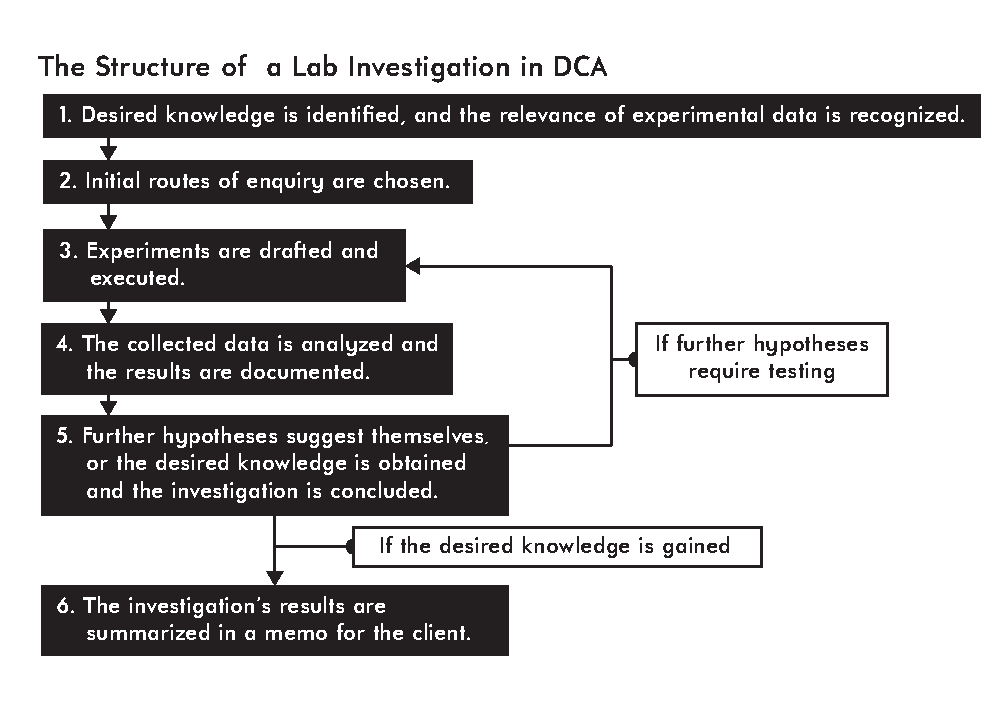
\includegraphics[width=1.2\textwidth]{Lab_Investigation_Diagram.pdf}
\caption{Investigation diagram.}
\label{fig:investigation_diagram}
\end{figure}
% What departments in DCA test their products?
All aspects of an investigation - from experiment design through to presenting the results to a client - are handled by engineers assigned to the associated project. 
\par
Engineers assigned to medical projects perform the majority of the lab work that takes place at DCA. Occasionally engineers working on fast-moving consumer goods (such as toothbrushes or lotion bottles) will run tests to compare design variations or verify performance relative to some baseline. In general, the timeframes and functional requirements of such products limit the relevance of extensive experimental investigations. Medical products, on the other hand, are subject to strict regulation relating to product failure modes, and must, therefore, be extensively tested.
\par
% When do they test them and why?
Tests can be conducted at any point in a product's development, however as can be seen in Figure \ref{fig:tests_per_quarter}, the rate of testing increases as a product develops and varies dramatically according to project stage. Towards a product's release date is when resolving minor performance issues becomes a worthwhile pursuit, exploration for future product variants becomes a possibility, and rehearsal for fast-approaching regulatory tests becomes essential.
\begin{figure}
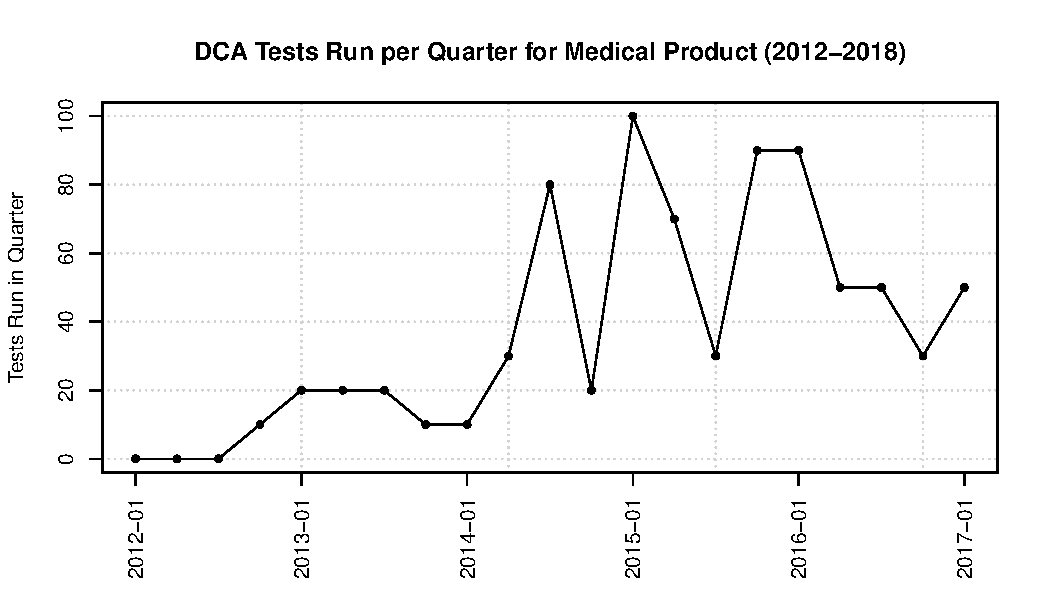
\includegraphics[width=\textwidth]{tests_per_quarter.pdf}
\caption{Testing frequency over the development of a single medical product.}
\label{fig:tests_per_quarter}
\end{figure}
\par
% How do they test them?
The equipment supporting this work includes axial and torsional testing machines, environment chambers, coordinate measuring machines, mass balances, and high-speed cameras, among other engineering instruments. Investigations commonly revolve around a particular experimental set-up, but other experiments are sometimes conceived to provide supplementary information. With that in mind, this report attempts to be data-agnostic in its recommendations of analytical techniques.
\par
DCA's engineers also apply statistics to are tolerance analysis and, increasingly, predictive user interfaces. Unfortunately, the latter cannot be discussed for confidentiality reasons; the former can be and is. Statistics is used to varying degrees within the Human Factors and upper management of DCA, but these applications are not reviewed here.
\par
To help make sense of how statistics is applied in DCA's lab investigations, each step of an experimental procedure is analyzed in turn. These steps are:
\begin{enumerate}
\item Planning and execution.
\item Analysis.
\item Presentation and visualization.
\end{enumerate}
Investigatory strategy guides the choice of all of the above and is examined in Subsection 2.2. For any experimental investigation to be successful, the experiments themselves need to be directed towards a purpose - in other words; the experiments need to be designed.

%%
\section{Experiment Design}
Experiment design can be used to make products that perform better, are more reliable, less risky to develop, and have a uniquely justifiable development process. Design of Experiments refers to both experiment designs and a broader philosophy of systematic experimentation. An experiment design is a particular structure of experiment; good experimental design produces data that is unambiguous and relevant to an experimental objective.
\par
Three principles form the backbone of robust experimentation:
\begin{description}
\item[Replication]{Testing a particular treatment on more than one unit. Replication allows experimental error to be estimated and, since unbiased errors cancel on being averaged, provides a more precise estimate of a treatment's effect.}
\item[Randomization]{Randomly allocating treatments to units and the sequence in which units are tested averages out the effects of nuisance variables, and validates the analytical assumption that observations are randomly drawn from a population.}
\item[Blocking]{Blocking accounts for the effects of nuisance variables when assigning treatments - units are grouped on the basis of a shared attribute, then treatments are distributed evenly among the groups. See Figure \ref{fig:blocking} for further explanation.}
\end{description}
These principles constitute the makings of any well-designed experiment, and they are evident in DCA's labwork: units are blocked according to factors such as component batches and time of assembly, testing and assembly sequences are randomized, and engineers are keen to provide replicates in their tests. The experimental designs used in the company are enumerated, explained, and critiqued in Table \ref{tab:exp_designs}.
\par
Despite the company's awareness of these fundamental aspects of experiment design, there is a tendency to forget to consider how the data collected will be analyzed when planning an experiment, and to think about how to structure an investigation. Analysis should be considered from during the planning stages since it is what will make apparent the test's outcome. By thinking about how the collected data should be analyzed, possible confounding factors can be identified and controlled.
\par
DCA also lacks a framework for planning experimental investigations. As a consequence of this, basic activities such as verifying that experimental set-ups produce repeatable results, scoping an investigation, and running screening experiments to close off unpromising avenues of enquiry are routinely forgotten. The dominant experimental strategy within the company is a best-guess approach: one treatment is tested in each experiment, chosen based on the expert insight of the engineering team. This method's greatest shortcoming is that if the treatment does not elicit the desired effect, then the next factor to vary must be guessed at, a process that can continue almost indefinitely. Furthermore, if a treatment is successful, then its investigation may be concluded when in fact a better solution exists.
\par
\begin{figure}
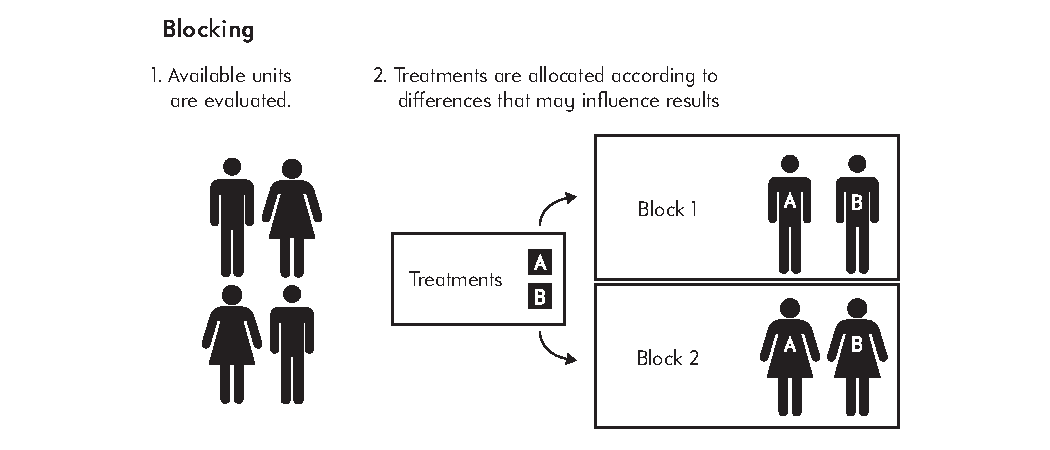
\includegraphics[width=\textwidth]{Blocking.pdf}
\caption{Diagram of what blocking involves.}
\label{fig:blocking}
\end{figure}
\par


\renewcommand\arraystretch{1.5}
\begin{table}[H]
\hspace*{-2.25cm}
\small
\centering
	\begin{tabular}{p{3.5cm} p{6cm} p{6.5cm}}
	\toprule
	\textbf{Experimental Design} 		& 	\textbf{Description}	&	\textbf{Evaluation} \\\toprule
	Randomized complete block design	 & 	The units are split into blocks according to differences that may influence the response, then each treatment is randomly assigned to at least one unit from every block. &  Allows the effects of nuisance variables to be eliminated during analysis, provided the block factor and treatment do not interact. \\
	& & Lends itself to established analytical techniques (e.g. ANOVA). \\
	& & Can be extended to block on more than one factor (such a design is called a Latin square) \\
	& & Not possible if the number of units in a block is fewer than the number of treatments to be tested. \\
	&&\\
	Factorial design & The factors and their respective levels are chosen, then all possible combinations of the factors are tested. & More time-efficient than testing one factor per experiment. \\
	& &  May be limited by resources if there are many factors \\
	& & Allows interaction effects to be estimated.
	\\\bottomrule
	\end{tabular}
	\hspace*{-2.25cm}
	\caption{Experimental designs applied in DCA.}
	\label{tab:exp_designs}
\end{table}

After an experiment is designed, it must be run. As has been mentioned, DCA is well endowed to run experiments, and has a system in place for documenting the date, purpose, and conditions of an individual experiment. These documents are scanned and stored on a local network, where they can be referred to at a later date. These documents are useful, but could be improved by:
\begin{itemize}
	\item Listing what factors were controlled and which were uncontrolled. This would help future users of the test data avoid mistakes when interpreting results.
	\item Providing a reference to a test in which the experimental apparatus and procedure used was verified.
	\item Including an image of the experiment so that the experiment can be understood by other engineers.
	\item A specific statement of how the collected data will be analyzed. This is to ensure that the results of an experiment are used in the way intended by the overall investigation.
\end{itemize}

Once an experiment has been planned and executed, it remains to analyze the raw data to extract useful information.

\vspace{48pt}
%%
\section{Analysis}
Analyses in DCA rely heavily on expert knowledge of the systems being tested and rarely on statistical results. This is probably because the relevance of statistics may not be clear, and how it might be applied even less so, which is understandable. It is widely agreed that most people's experience with statistics is one of discomfort and bemusement. Having said this, relying on intuition alone risks falling prey to cognitive biases, missing valuable information that isn't superficially obvious, and being unable to relate physical behaviours to experimental observations. Foregoing statistics when analyzing product behaviour handicaps the ability of an engineer to design a robust product.
\par
The reports surveyed contained summary statistics, such as arithmetic means, variances, maximums, minimums, and so on. A few made use of interval estimates as informed by a regulatory standard, and one report applied a t-test. These tools will now be explained, and their usefulness and possible weaknesses detailed.
\par
\subsection*{Summary Statistics}
 Randomness refers to variation in a response as a result of uncontrolled factors. If a coin is always flipped according to the same process, then it will always land in the same orientation. By contrast, if a coin is flipped by hand, then the person doing the flipping has a limited amount of control over the factors affecting the flip. As a result, there is uncertainty as to what the outcome of that flip will be. There are two ways to reduce this uncertainty: Either make assumptions about how those flip-influencing factors vary or measure them. Assumptions allow real-world knowledge to dictate what outcomes are possible what their relative propensities are. Conversely, measurements allow factor effects to be estimated, accounting for the sources of variation in the response.
 
  The assumption of normality, for example, is wielded as a claim many independent effects, no one of which is especially large, are responsible for a response's variation (See the Appendix). Alternatively, it may be suggested that no particular outcome is favoured by a system, in which case uniformity could be assumed. In both instances, a distribution of outcomes is assumed based on physical knowledge, making it possible to analyze the system for useful information.
 
Mathematical analysis can be used to understand systems that vary randomly. As with any theory, some tools need to be defined to make the maths possible: a random variable is one of these tools. Despite its name, a random variable (r.v.) is in fact a function that maps events onto real numbers. For example, we could define an r.v. $X$ that maps the outcomes of a coin toss onto the numbers 1 and 0:
 \begin{align}
	X(\texttt{Coin lands Heads}) = 1 \\
	X(\texttt{Coin lands Tails}) =0
 \end{align}
Usually, the choice of mapping is quite natural - for example, we might use an r.v. that counts the number of successes in many trials, or that takes on the value of a measurement. 
\par
Variation in the events that an r.v. maps from is described using a probability distribution. Each value is weighted according to its probability or, in the case of continuous-valued r.v.s, the ratio of the width of an interval of values to its probability. Figure \ref{fig:example_pd} highlights this difference.
\begin{figure}[h!]
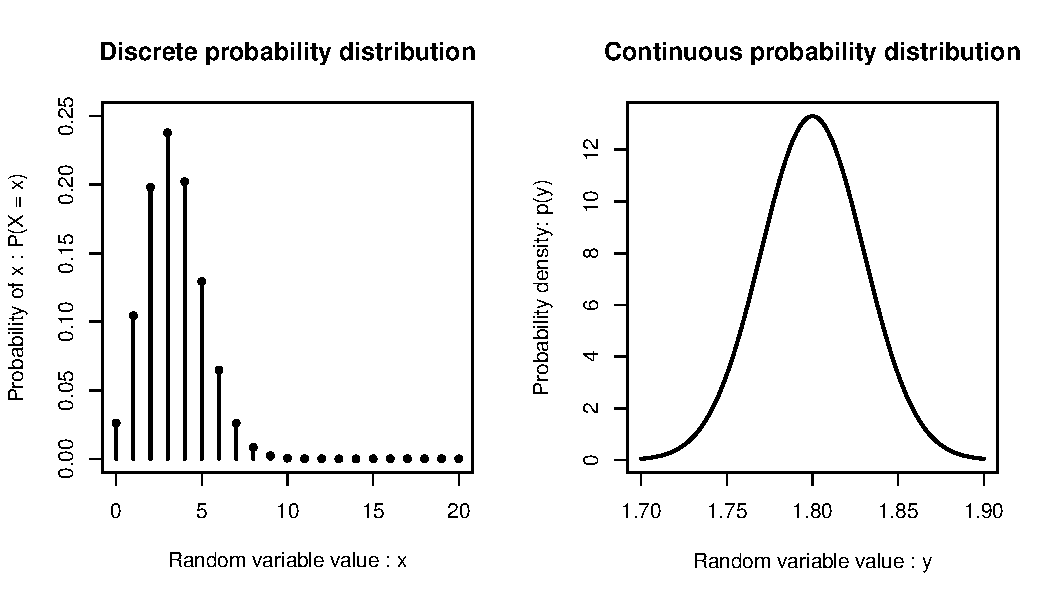
\includegraphics[width=\textwidth]{probability_distributions.pdf}
\caption{Left: Probability mass function. Right: Probability density function.}
\label{fig:example_pd}
\end{figure}
\par
The essential problem of experimental statistics is trying to understand the distribution of a random variable from just a sample. In product design, this means using measurements from just a limited number of prototypes to estimate the behaviour of a much larger number of units. The attributes of a random variable's distribution - such as its spread and average - can be estimated using summary statistics.
 \par
A sample's mean response, for example, approximates the mean response of a larger population of units. DCA use sample means to discriminate between the performance of two or more populations, each representing possible design variants. The sample mean's accuracy improves as more samples are tested, with diminishing returns, a relationship that is shown in Figure \ref{fig:se_with_sample_size}. A sample may not be representative of its population, so it is sensible to estimate how far a sample mean is likely to be from the population mean. Bigger samples tend to represent their populations better, and tightly clustered responses imply that any one response is likely to be close the population mean. The standard error of the sample mean - the average difference between a sample mean estimate and the population mean - reflects these observations, as it corresponds to $\frac{\sigma}{\sqrt{n}}$, where $\sigma$ is the standard deviation of the population and $n$ is the number of units in the sample.
\begin{figure}[h]
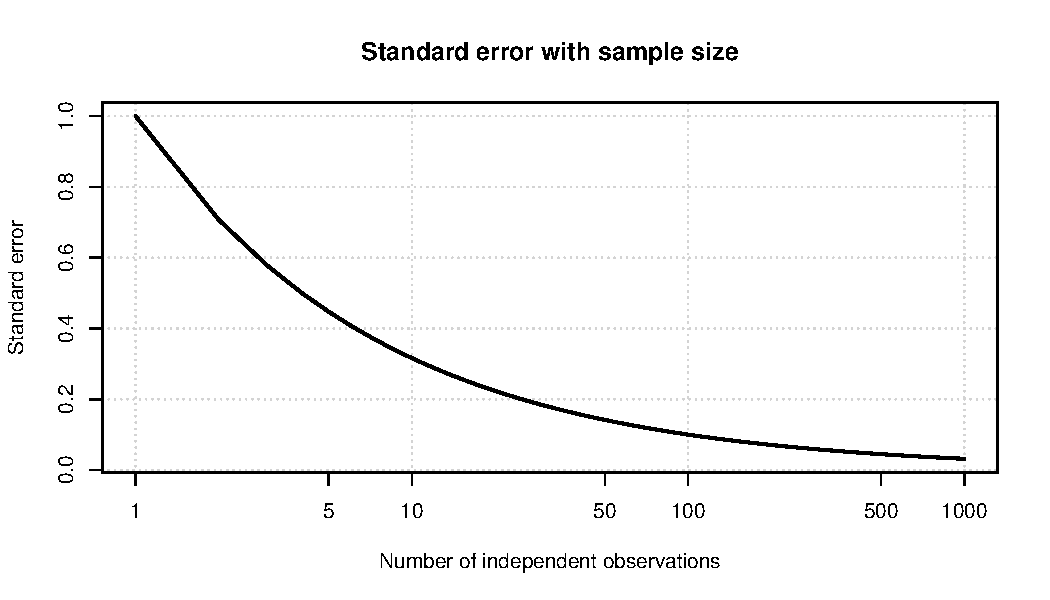
\includegraphics[width=\textwidth]{se_with_sample_size.pdf}
\caption{As sample size increases, the sample mean will - on average - draw closer to the population mean.}
\label{fig:se_with_sample_size}
\end{figure}

Certain summary statistics can be thought of as estimates of a distribution's parameters. These are values that constrain a particular distribution's shape. The normal distribution's shape, for example, can be specified by supplying just two values: the variance (spread) and mean (location). The uncertainty inherent in test results is accurately presented by estimating a parameter's distribution, which will capture the amount of certainty warranted by a test. This is not the case for small-sample point estimates. DCA's engineers are particularly at risk of the latter because their experiments are constrained by the number of units that can be tested. Consequently, Section \ref{suggested_methods} contains tools for making distributional estimates.

 Estimating a distribution will be seen again later, in the section on Bayesian inference. Interval estimation is an alternative method for quantifying uncertainty: Its results need to be interpreted carefully, and its assumptions need to be verified.

\par

\newpage
\subsection*{Tolerance Intervals}
DCA's base their most sophisticated statistical analysis on ISO 16269-6, \emph{Determination of statistical tolerance intervals}. This standard outlines how to construct tolerance intervals under either no assumptions about the random variable's distribution, or the assumption that the random variable is normally distributed.
\par
 A tolerance interval is a range of values that's likely to contain a particular fraction of the population. Because this interval is an estimate, it can only contain the advertised fraction of the population some of the time. The proportion of intervals that would, on average, contain the specified fraction of the population is called the confidence level. If many $99\%$ tolerance intervals were constructed for different samples of the same size to a $95\%$ confidence level, then $95\%$ of the intervals estimated would contain at least $99\%$ of the population. Figure \ref{fig:tolerance_intervals} demonstrates this use case.
\begin{figure}[h]
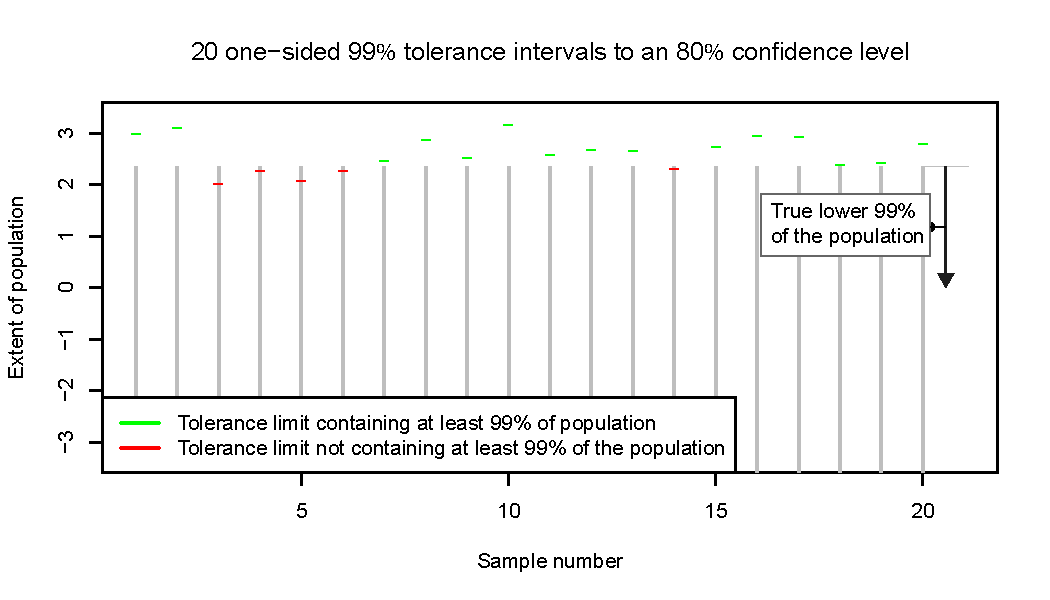
\includegraphics[width=\textwidth]{tolerance_intervals_2.pdf}
\caption{Tolerance intervals estimate where the bulk of a population lies.}
\label{fig:tolerance_intervals}
\end{figure}

DCA used tolerance intervals in to check that a given proportion of a population satisfied a performance threshold. Their use was not widespread, and in some of the reports studied the $k$-values\footnote{A $k$-value is a term used in the ISO standard to represent the number of sample standard deviations from the mean that will contain at least $p\%$ of the population $(1 - \alpha)\%$ of the time, where $(1 - \alpha)$ is the confidence level.} were incorrectly calculated. Furthermore, no efforts were made to test the assumption of normality.

The strengths and suggestions for DCA's tolerance intervals are listed in Table \ref{tab:tol_intervals}.
\begin{table}
\caption{Evaluation of tolerance intervals.}
\small
\hspace*{-.5cm}
\begin{tabular}{p{6.5cm}p{6.5cm}}
\toprule
\textbf{Strengths}	&	\textbf{Shortcomings} \\
\toprule
Provides a threshold indicating roughly where a certain fraction of the population is. & Confidence levels can be misinterpreted as specifying the probability that a constructed interval contains at least $95\%$ of the population. \\
In line with the expectations of regulatory standards. & If normality is assumed, it needs to be checked. \\
Can be applied without theoretical understanding. & Repeated use at a low confidence level increases the probability that the limit will be under-estimated. \\
& k-values need to be looked up, which could easily be done incorrectly if the theory isn't understood.\\
\bottomrule
\end{tabular}
\label{tab:tol_intervals}
\end{table}

\newpage
% Confidence intervals
\subsection*{Confidence Intervals}
Another tool that DCA's engineers occasionally use is confidence intervals, which indicate a range of values that a parameter is likely to fall within. As with tolerance intervals, this range will only contain the population parameter a certain fraction of the time, a problem that's unavoidable since there will always be a chance that an unrepresentative sample is drawn. For example, if we were to construct a confidence interval for the population mean of 100 samples, each of 5 units, the confidence level would tell us how many of these intervals would - on average - contain the actual value of the population mean. Figure \ref{fig:confidence_intervals} demonstrates this idea. Confidence intervals can be placed on any parameter estimate, although they are most commonly used to quantify the uncertainty on an estimate of the population mean. Their derivation is similar to a tolerance interval's and is in the Appendix.

\begin{figure}[H]
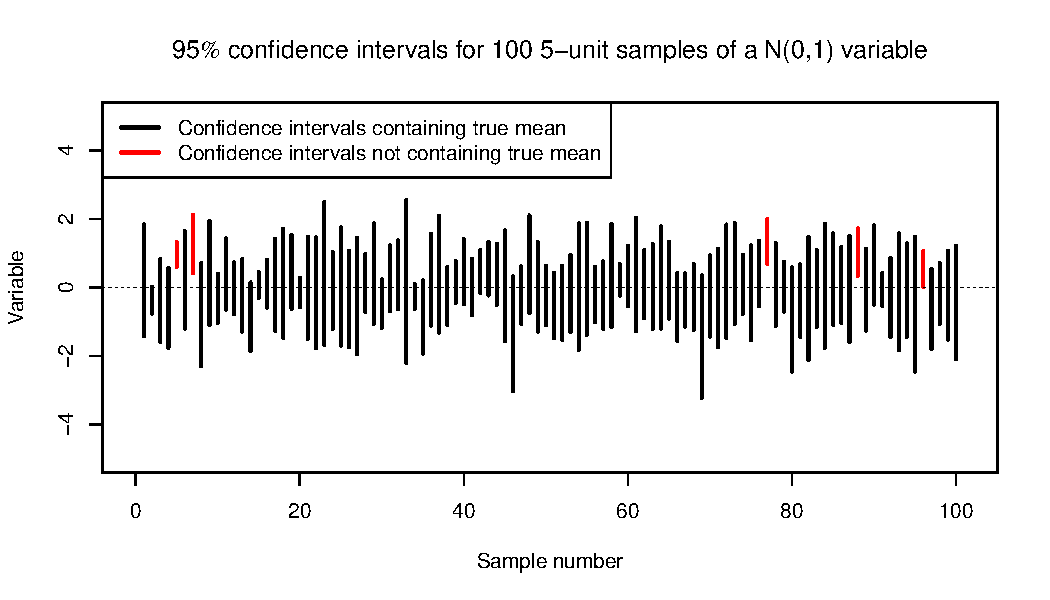
\includegraphics[width=\textwidth]{confidence_intervals.pdf}
\caption{Confidence intervals indicate the range of values likely to contain an estimated parameter.}
\label{fig:confidence_intervals}
\end{figure}
Confidence intervals suffer from similar problems to tolerance intervals. DCA's engineers use them very rarely, meaning they make decisions with a limited appreciation of the uncertainty in their estimates. If only large differences in effects are of interest, this is not a substantial problem. However, if subtle differences are important, or sample sizes are limited, then it is necessary to quantify an estimate's uncertainty so that erroneous or inappropriately confident conclusions are not made.

\subsection*{Monte Carlo Estimation}
Monte Carlo estimation approximates a quantity by simulating the random process generating it. In DCA it was used to analyze tolerance chains in products. The use case was somewhat similar to the following: a gap between two components affected a product's function, so the distribution of possible gap values needed to be known. Several part dimensions influenced the gap's size, each of which had a distinct distribution describing its variation. Rather than attempt to derive the distribution of the gap's size directly, a computer was used to simulate draws of each dimension, then calculate a value for the gap that resulted. The relative frequencies of the simulated values were then used to approximate the distribution of the gap's size, from which properties such as its mean and variance could be estimated. Figure \ref{fig:monte_carlo} is a diagram of this process.
\begin{figure}[h!]
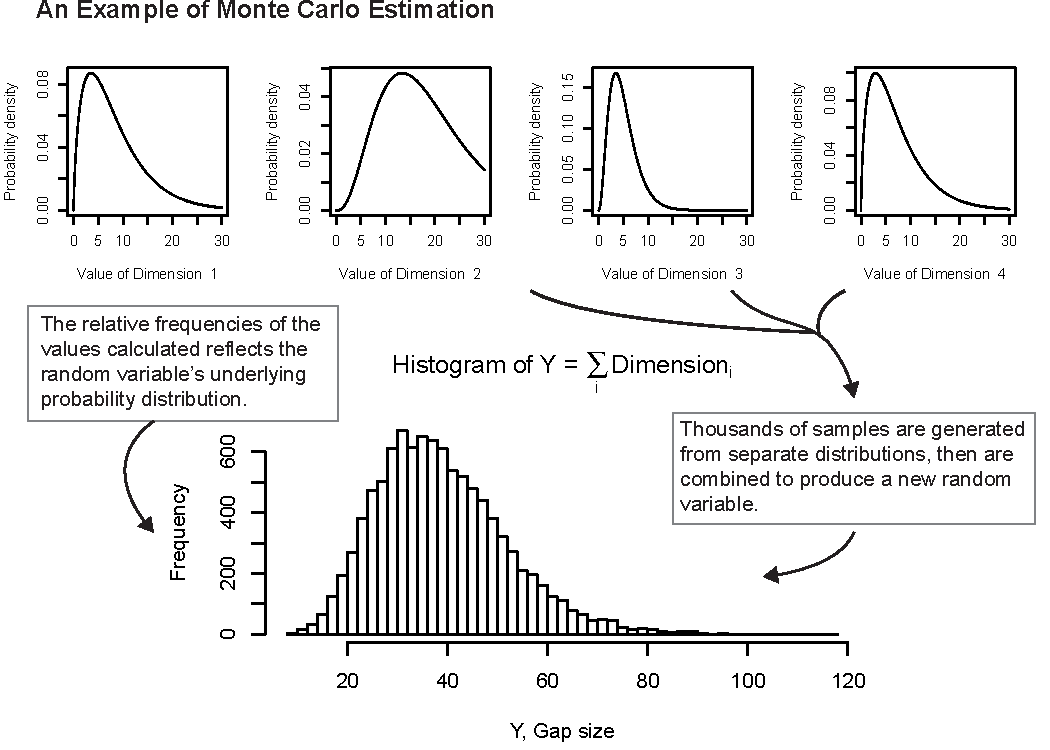
\includegraphics[width=1\textwidth]{MC_estimation.pdf}
\caption{Process diagram for a Monte Carlo simulation.}
\label{fig:monte_carlo}
\end{figure}

Monte Carlo estimation is a powerful statistical tool that is easily implemented and interpreted. Enlarging its use beyond tolerance analysis to other areas of work at DCA would allow the effects of variation in manufacturing processes on product performance to be predicted, and hypothesis tests to be run by engineers with limited statistical training. Mathematical models were used in the company to analyze a product's performance: randomly sampling the inputs to these models would give DCA's engineers the ability to profile the overall variation in performance, rather than estimate the worst or best case alone. Monte Carlo methods can also be used to conduct hypothesis tests; by considering the probability of the observed sample as indicated by a distribution of samples generated via MC methods.

\newpage
\section{Visualization}
\label{sec:dca_vis}
Visualization is essential to clearly and convincingly summarizing an experiment's results. Graphical tools allow engineers and clients to see for themselves what's been discovered. A plot should be relevant, easily interpretable, and accurately convey its underlying data.
\par
DCA's reports and client presentations contain plots of experimental data generated using either Microsoft Excel or Matlab. These plots are line or bar charts, along with the occasional scatterplot. Line charts are frequently used in DCA because they are directly plottable from the raw data output by their axial and torsional testing machines. Bar charts, on the other hand, tended to be used to highlight differences between groups, such as their means or maximums. Scatter plots were used specifically to present tolerance intervals relative to a set of performance criteria, as is shown in Figure \ref{fig:tolerance_intervals_plot}.
\begin{figure}[h!]
	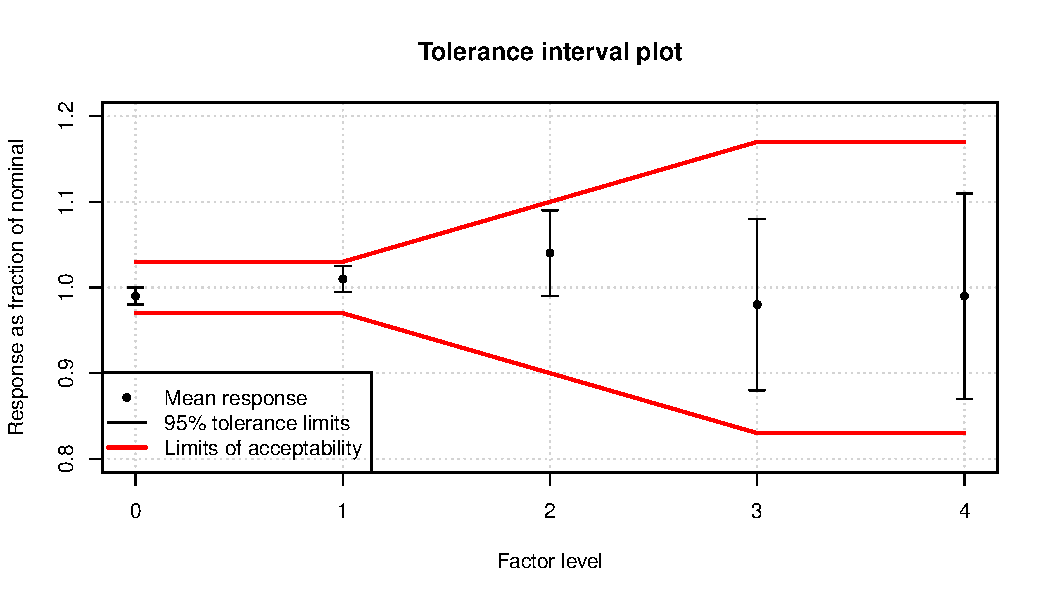
\includegraphics[width=\textwidth]{tolerance_intervals_plot.pdf}
	\caption{Tolerance interval plot.}
	\label{fig:tolerance_intervals_plot}
\end{figure}

Directly plotting raw data requires very little time, and results in plots that are easily related to patterns observed over the course of an experimental run. These are major benefits in favour of using line charts to understand the results of an experiment quickly. However, there are several reasons why these types of charts are not suitable for presenting at team meetings, or to clients. Figure \ref{fig:line_chart} was taken from a DCA test report and is of a type that was used regularly in team meetings. In this test, the response of the units at 10.8 seconds was of interest, yet all raw data was plotted. Plotting irrelevant data has various negative corollaries: the redundant information away from 10.8 seconds is distracting and of limited use, since it is not possible to see how individual units are behaving.  Even if the other displacements were relevant, the plot would still be somewhat misleading as attention is directed to the group extremes, and cannot be used to see anything besides gross differences between groups. Moreover, line charts can conceal the actual resolution of the data collected, particularly if a spline fit or graphical smoothing has been applied\footnote{Excel automatically smooths line charts.}. Subsection \ref{suggested_vis} suggests solutions to these problems.
\begin{figure}[h!]
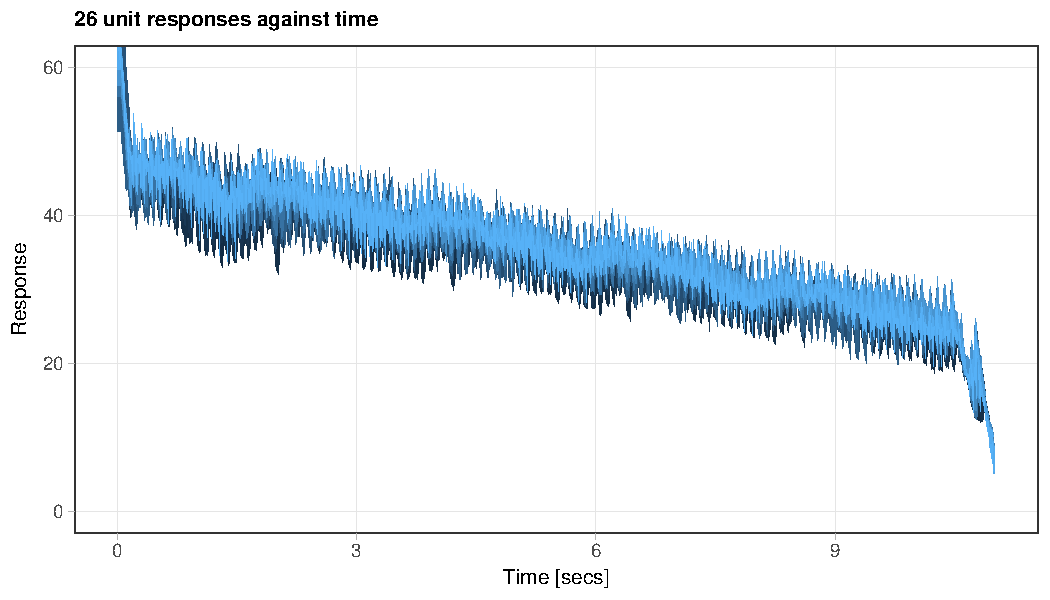
\includegraphics[width=\textwidth]{imitation_line_chart_2.pdf}
\caption{A representative use of line charts from a DCA test report. Each shade of blue corresponds to a unique unit.}
\label{fig:line_chart}
\end{figure}

As has been mentioned, bar charts and scatter plots were also used within DCA, albeit less frequently than line charts. There are several ways in which the use of these tools could have been improved. Plotting errors bars on bar charts would allow the uncertainty in the estimates to be represented, making group comparisons less prone to unwarranted confidence. Alternatively, the individual unit responses could be included as a scatter plot to give the audience a sense of the sample size used and response variance. Scatter plots are capable of displaying location, spread, density, and sample size information, making them a valuable tool for summarizing experimental data: the response at 10.8 seconds in Figure \ref{fig:line_chart} could easily be captured for each unit then presented in a scatter plot, resulting in a plot that is easier to read and discuss.


\section{Review}
The report so far has presented and critiqued the statistical methods used by DCA's engineers at each step in an experimental procedure. Planning of experimental investigations has also been detailed, as has its weaknesses. The next section suggests methods that will help DCA use statistics more effectively by:
\begin{itemize}
\item Estimating distributions of plausible parameter values rather than their ``most-likely'' or ``worst-case'' values.
\item Planning investigations that systematically identify the main factors influencing a response, and the factor levels needed to optimize that response.
\item Using regression to relate factors to a response.
\end{itemize}
Why these are desirable is explained in the sections to come. In short, they were chosen to:
\begin{itemize}
\item Allow a product's behaviour to be methodically analyzed and optimized.
\item Represent the uncertainty associated with experimental work more intuitively and transparently.
\end{itemize}
Table \ref{tab:exp_procedure} compares DCA's experimental procedure against conventional experimental steps.

\begin{landscape}
\vspace*{-3cm}
{\tiny
\begin{longtable}{p{4cm} p{7cm} p{6cm} p{6cm}}
\caption{Comparison of DCA's experimental procedure with conventional practice.}\\
\toprule[0.15em]
\textbf{Experimental step} & \textbf{DCA's implementation} & \textbf{Strengths} & \textbf{Suggestions} \\
\toprule[0.15em]
Recognition and statement of the problem. & Problems in need of experimental work were identified in either other experiments or design-side activities. These problems were not formally stated, but were agreed in loose terms among the engineering team. & The benefits that experimental investigations provide, such as empirical validity and flexibility, were recognized. & A precise problem statement would focus investigations towards a particular end, and allow progress towards that end to be gauged. It would also make it clear to the team, client, and management, exactly what an investigation aims to achieve. \\ 
 &  &  & Specific problem statements would have made it easier to review previous work - without them, it was difficult to determine where one investigation began and another ended. \\ 
\cmidrule{1-4}
Choice of factors, levels, and ranges. & These choices were made in engineering team meetings, which occured weekly. Factors were identified haphazardly, which was detrimental to the course of investigations because it was sometimess unclear which nuisance variables a previous experiment had controlled. Ranges and levels were chosen according to expert knowledge. The number of levels tended to be small (2 or 3) because differences rather than overall responses were of interest. & The level choices were well-justified using either physical reasoning or previous experimental results. & Monitoring which factors are controlled and uncontrolled would allow a response's variation to be broken down into its components , and would improve the validity of the data collected.\\ 
 &  & Deciding which factors are relevant in a meeting used the entire team's engineering knowledge and critical thinking skills. & A meeting should be a place to review a choice, not to make it - conversation is not methodical and can easily miss relevant information.\\
 & & Stating whether factors are controlled would avoid mistakes when interpreting results. \\ 
\cmidrule{1-4}
Selection of the response variable. & The response variable would be mentioned on an experiment's cover sheet (e.g. torque output of mechanism), but its relation to the investigation's objective was not always documented. More than one way to measure the response variable would almost always be considered. & Engineers in the company could generate many possible response variables, and analyze their respective merits. & Precursor experiments comparing the candidate response variables may reduce the length of investigations. \\ 
 &  & The response variable chosen is chosen carefully to closely represent the system under study. & Documenting the alternative response variables would make it easier to clearly outline why one method is superior, and to transition between testing methods as circumstances change. \\ 
\cmidrule{1-4}
Choice of experimental design. & Experiments are designed within meetings. They will involved randomization, replication, and blocking, but do not take advantage of formal experiment designs suited to particular problem constraints (e.g. resource limitations). The desired analysis is not stated beforehand, and the majority of tests are comparative. & Simple experiment designs are easily communicated, executed, and documented. & A well-chosen experimental design can reduce the resources (time, materials, and effort) expended in satisfying the investigation's objective. \\ 
 &  &  & Considering analysis beforehand makes it possible to ensure analytical assumptions are met. \\ 
\cmidrule{1-4}
Performing the experiment. & Experiments are run in on-site laboratories. Frequently run experiments have protocols; hand-written observations and summaries of important information (date, experimenter, purpose etc.) are mandatory for all experiments. & Labs provide experimental control over nuisance variables. & Experimental fixtures should be shown to generate repeatable, reliable results before being used. \\ 
 & & Images of test set-up would make it much easier to retrospectively understand an experiment. \\ 
 &  & Experiments are run by engineers solving the problem - this makes engineers personally responsible for their results, and exposes them to undocumented experimental information. \\ 
\cline{1-4}
Analysis of the data collected. & Analyses were run as soon as data is available, and were handled by the engineer that conducted the experiment. Excel - and occasionally Matlab - were used to analyze test data. The conclusions resulting from analyses tended to be judgemental as opposed to statistical. Compared to the time spent running the experiment, analysis was brief, and the lack of forethought about an appropriate form of analysis meant that analytical conclusions were sometimes lacking. & Engineering expertise was applied to explain experimental results in a physically meaningful way. & Statistics should have been used more regularly ensure that sound analytical conclusions were drawn - subjective assessment alone is susceptible to various biases that can lead to lost time and confusion.\\ 
 &  &  & More time should be allocated to analysis in experimental investigations. Of the one-hundred or so test reports surveyed, very few of them did more than plot line charts of the raw data: analysis is crucial for an experiment to be useful, and neglecting to spend invest time in it can mean that dozens of experiments are run when a few would suffice.\\ 
\cmidrule{1-4}
Conclusions and recommendations & Experimental conclusions were presented to clients via presentations, memos, and technical reports. Interim results were presented every week in team meetings. & The importance of graphics was realized and put to good effect in client presentations. & Charts exist beyond those currently being used that may make it easier to explain investigation outcomes. \\ 
 &  \\
\bottomrule
\label{tab:exp_procedure}
\end{longtable}
}
\end{landscape}


\newpage
%%  SUGGESTED METHODS %%
\chapter{Suggested Methods}\label{suggested_methods}
\label{chap:modernstats}

Having assessed DCA's current use of statistics, it is possible to suggest methods from modern statistical practice that would give them new capabilities and improve their existing ones. Like Section 2, this section is categorized by the steps in an experimental process.


\newpage
\section{Analysis}
\subsection*{Regression Analysis}
% What's a regression model?
% How's it useful to DCA?
% What do they consist of?
% What are their limitations, and how can they be applied to more difficult problems?
Experimental work often tries to an answer questions such as:
\vspace{-10pt}
\begin{itemize}
\item Which factors are having a big effect on the response?
\item How does a factor affect the reponse? How do several factors interact?
\item Which design variation is better?
\end{itemize}
\vspace{-10pt}
 Regression analysis would allow DCA's engineers to answer questions like these. Knowing what parameters affect the product, and by how much,  focuses development on the things that matter, resulting in a better quality product that's less risky to develop.
 \par
 Regression estimates how a continuous response changes with some inputs. Linear regression uses a linear function to predict the reponse: This may sound limiting, since in real life lots of relationships are nonlinear, but nonlinear relationships can be made linear by transformation.
\par
  Linear models describe a response $y$ as a linear function of some parameters $\hat{\beta}_i$, each weighted by a corresponding input $x_i$. The rate of change of the response with respect to a particular input is embedded in that input's parameter. An example of such a model would be:
\begin{equation}
	\hat{y} = f(x_1, x_2) = \hat{\beta}_0 + \hat{\beta}_1 \cdot x_1 + \hat{\beta}_2 \cdot e^{x_1}+ \hat{\beta}_3 \cdot x_1 \cdot x_2
\end{equation}
Where $\hat{y}$ is the estimated response, $x_i$ is an input, and $\hat{\beta}_j$ is the coefficient of the $j$th input. Note that while the coefficients $\hat{\beta}_j$ are linear, the predictors $x_j$ can be nonlinear functions of the measurements.

This model can be fit by adjusting the $\hat{\beta}_i$ values so that $\hat{y}$ is a good estimate of the true response. To do this, it is necessary to measure how inaccurate $\hat{y}$ is relative to $y_i$. One way of measuring fit inaccuracy is the residual sum of squares:
\begin{equation}
	\text{RSS}(\hat{\beta}) = \sum_{i = 1}^m \Big(y_i - \sum_{j = 1}^p \hat{\beta}_i x_{ij})^2
	\label{eq:rss}
\end{equation}
Where $y_i$ is the response of the $i$th example, and $x_{ij}$ is the $j$th predictor value of the $i$th example. This measure of fit is a good one for several reasons, the most intuitive of which is that it minimizes the overall distance between the estimates $\sum_{j = 1}^p \hat{\beta}_j x_{ij}$ and the responses $y_i$ \footnote{The residual refers to the difference between an estimated response and a true response at a particular set of inputs. Error refers specficially to deviation of a response around its expected value.} . There are two alternative justifications for least squares, which are both presented in the Appendix.

 Figure \ref{fig:linear_regression}. 
\begin{figure}
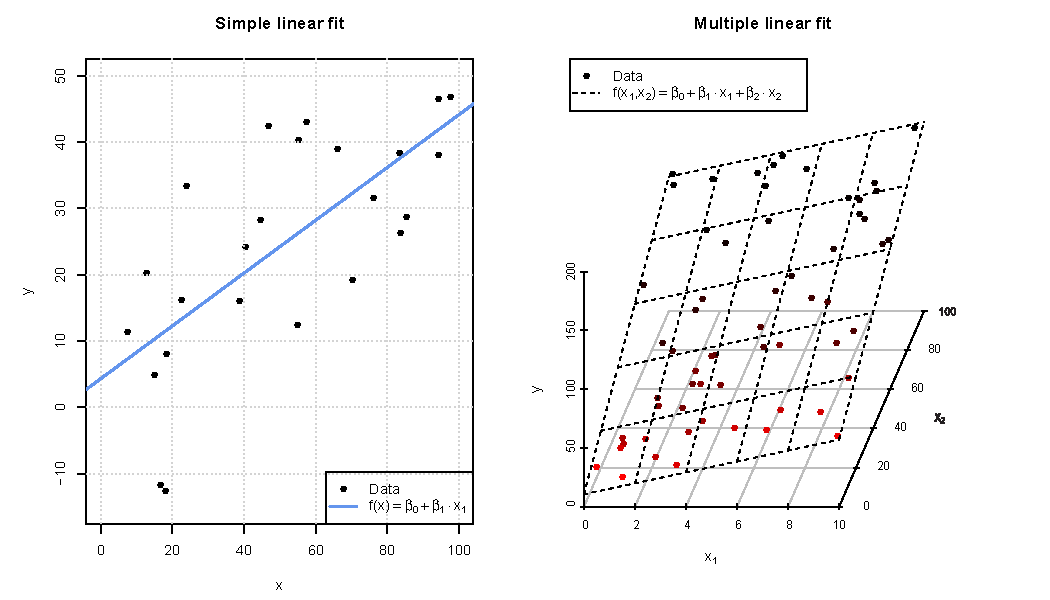
\includegraphics[width=\textwidth]{linear_fits.pdf}
\caption{A simple and a multiple linear fit.}
\label{fig:linear_regression}
\end{figure}

From a practical standpoint, regression models should be fit using software. Matlab, R, or Octave can all be used to fit regression models. By setting up the problem such that the $N$ observed responses are in a column vector $\mathbf{y}$, their associated $p$ inputs form the rows of a matrix $\mathbf{X}$, which is $N \times p$, and the $p$ coefficients are in a column vector $\hat{\beta}$, it is possible to succinctly write the RSS criterion, then minimize it:
\begin{align}
	\text{RSS}(\hat{\beta}) &= (\mathbf{y - X}\hat{\beta})^T(\mathbf{y - X}\hat{\beta}) \\
	\frac{\partial \text{RSS}}{\partial \hat{\beta}} &= -2\mathbf{X}^T(\mathbf{y - X}\hat{\beta}) = 0 \\
	\implies &\hat{\beta} = (\mathbf{X}^T\mathbf{X})^{-1}\mathbf{X}^T \mathbf{y} \label{eq:normal_eqtn}
\end{align}

As a case study to show why linear models are useful, consider a test in which the load delivered by three groups of ten units is measured. The differences between the groups are categorical: the groups correspond to three design variations $A, B,$ and $C$. Since there isn't a natural order to the variations, it is necessary to encode this difference in a sensible way. There are several ways to do this, and a simple indicator stating whether a unit has a particular modification is sufficient. Table 5 shows this encoding. As will hopefully become apparent, choosing how to encode categorical variables matters a good deal with regards to how the regression coefficients beta should be interpreted.
\begin{table}
\centering
\caption{Dummy coding of groups.}
\small
\begin{tabular}{c c c c c}
\toprule
\textbf{Unit ID}                 & $\mathbf{x_A}$ & $\mathbf{x_B}$ & $\mathbf{x_C}$ & \textbf{Load, $\mathbf{y}$ [N]} \\
\midrule
1                       & 1 & 0 & 0 & 5.43         \\
2                       & 0 & 1 & 0 & 7.48         \\ 
& & \vdots & & \\
30 & 0 & 1 & 0 & 6.47 \\
\bottomrule
\end{tabular}
\end{table}

Next the model is set up:
\begin{gather}
	\hat{y} = \hat{\beta}_0 x_A + \hat{\beta}_{1}x_B + \hat{\beta}_{2}x_C = x \hat{\beta} \label{eq:categorical_regression} \\[5mm]
	\mathbf{X} = 
		{\tiny
			\begin{bmatrix}
				x_1 \\ x_2 \\ \vdots \\ x_{30}
			\end{bmatrix}
			=
			\begin{bmatrix}
				 1 & 0 & 0 \\  0 & 1 & 0 \\ \vdots & \vdots & \vdots \\ 0 & 1 & 0
			\end{bmatrix}}
	\quad \mathbf{y} = {\tiny \begin{bmatrix} 5.43 \\ 7.48 \\ \vdots \\ 6.47 \end{bmatrix}}
	\quad \hat{\beta} = {\tiny \begin{bmatrix} \hat{\beta}_0 \\ \hat{\beta}_1 \\ \hat{\beta}_2 \end{bmatrix}}
\end{gather}
We can then use the normal equation (Equation \ref{eq:normal_eqtn}) to make the least-squares fit. As it happens, in this case $\hat{\beta}_A$, $\hat{\beta}_B$, and $\hat{\beta}_C$ are the average responses of each group, as is shown in Figure \ref{fig:categorical_regression}.
\begin{figure}[h]
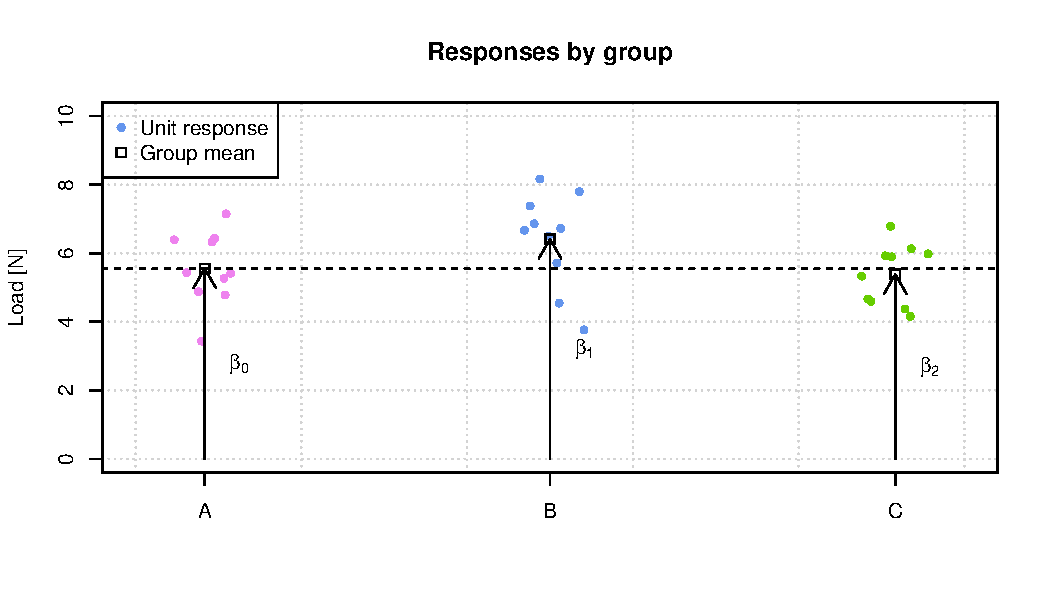
\includegraphics[width=\textwidth]{categorical_regression.pdf}
\caption{Unit responses by group.}
\label{fig:categorical_regression}
\end{figure}

Figure \ref{fig:alt_categorical_regression} shows how the meaning of the regression coefficients could change with choice of encoding. Whereas in Equation \ref{eq:categorical_regression} the fit coefficients were estimates the group means, the coefficients here correspond to the model:
\begin{equation}
	\hat{y} = \hat{\beta}_0 + \hat{\beta}_1x_B + \hat{\beta}_2x_C
\end{equation}
The practical implication of this is that $x_B$ or $x_C$ are now indicator variables for whether a unit deviates from the mean response $\hat{\beta_0}$.
\begin{equation}
	\text{RSS}(\hat{\beta}) = \quad
					\smashoperator{\sum_{i: x_i \in \{x: x_a = 1\}}}(y_i - \hat{\beta}_0) \quad + \quad
					 \smashoperator{\sum_{i: x_i \in \{x: x_b = 1\}}}(y_i - (\hat{\beta}_0 + \hat{\beta}_1)) \quad + \quad
					 \smashoperator{\sum_{i: x_i \in \{x: x_c = 1\}}}(y_i - (\hat{\beta}_0 + \hat{\beta}_2))
\end{equation}
To minimize the first term, $\hat{\beta_0}$ can be set to group A's mean - the other two terms can be minimized by letting $\hat{\beta_1}$ and $\hat{\beta_2}$ correspond to the mean deviation of groups B and C from A.

 Something to be quite careful of is redundantly encoding the groups. If a constant term $\hat{\beta}_4$ were to be included in the model above, then there would be many equivalent ways to express the group effects: $\hat{\beta}_4$ could be any constant value, and $\hat{\beta}_1, \hat{\beta}_2, \hat{\beta}_3$ would be set to deviate from this constant to the group averages. This means that attempts to evaluate Equation \ref{eq:normal_eqtn} will be unsuccessful or unstable\footnote{The instability is caused by numerical errors in calculating the inverse directly.}.
 
\begin{figure}[h]
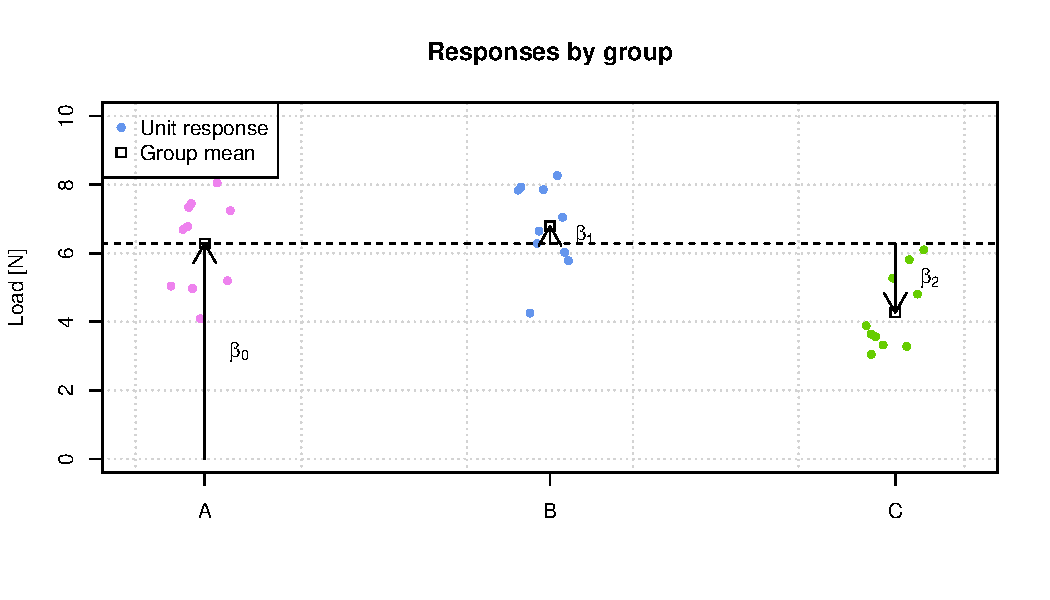
\includegraphics[width=\textwidth]{alt_categorical_regression.pdf}
\caption{Regression coefficients for alteranative categorical encoding.}
\label{fig:alt_categorical_regression}
\end{figure}

The fit of a linear model attempts to estimate the true relationship between the inputs and response. In other words, $\hat{\beta}$ are estimates of the parameters $\beta$:
\begin{equation}
	y = X\beta + \varepsilon
\end{equation}
Where $\varepsilon$ is the error in the response - variation caused by unmonitored variables. In the example, $\beta_1, \beta_2, \beta_3$ are the true group means, and $\hat{\beta}_1, \hat{\beta}_2, \hat{\beta}_3$ are estimates of them. These estimates are not going to be perfect, and their standard errors can be calculated to get a feel for how accurate they really are. To reemphasize, a standard error is the average difference between an estimate of a parameter over many samples, and the true parameter value. Standard error can be made smaller by reducing the group variance, or by making the sample sizes bigger.  DCA's engineers should seek to minimize variation that isn't relevant to the investigation because this will make it easier to see the effects of the inputs on the reponse for a given sample size. Calculation of standard errors is described and explained in the Appendix.

A reasonable criticism of the above example is that it is effectively just a drawn-out calculation of the group sample means. This is true, until the experiment is extended to involve another variable, this time a continuous one, say the volume of a lubricant applied to each design variant. Then the model can be adjusted to estimate the effects of the lubricant on the load output of each mechanism:
\begin{equation}
	\hat{y} = \hat{\beta}_0 x_A + \hat{\beta}_{1}x_B + \hat{\beta}_{2}x_C + \hat{\beta}_3 x_A x_l + \hat{\beta}_4 x_B x_l + \hat{\beta}_5 x_C x_l
\end{equation}
Where $x_l$ is the volume of lubricant applied, and $\hat{\beta}_3, \hat{\beta}_4, \hat{\beta}_5$ are the change in output force for each design variant per unit volume of lubricant. This model would allow an engineer to see not only how good design variants are relative to one another, but also how much lubricant would need to be applied to bring the performance of one in line with another. Linear models are powerful because they can be adapted to many situations, and because they provide a consistent way of disentangling the effects of experimental treatments.

As an aside, assessing the significance of differences between groups is frequently called Analysis of Variance (ANOVA). It is called this because the analysis focuses on decomposing variation into its sources. Two test statistics, the $t$ and $F$ statistics, can be used to run hypothesis tests on possible sources of variation. Under certain assumptions, these tests provide guidance as to whether a treatment induces an effect or not. It is relevant here because ANOVA can be viewed as linear regression with an emphasis on hypothesis testing. As discussed in the next section, hypothesis tests can be misleading. Furthermore, in complicated models, the canned formulae provided by some statistics resources, certain websites in particular, can become unwieldy and confusing, which could make its results suspect and difficult to explain. By contrast, the structure and basic principles of a linear model are consistent across a variety of model sizes. For this reason, it is suggested that DCA focus on learning to use linear models rather than attempt to use ANOVA.

Linear models would be useful to DCA because they can be used to figure out where variation in a response is coming from, which is the fundamental objective of most experiments. Identifying the factors that have the largest effect on performance, and quantifying those effects, is the first step in understanding how to change a design to make it both better-performing and more robust. Used in combination with multiple-factor experiment designs, linear models could reduce the time and resources taken to conclude an experimental investigation, and would offer a tool for aligning theoretical understanding with empirical evidence.

\newpage
\subsection*{Bayesian Inference}
% What is Bayesian inference?
% How can it be useful to DCA?
% What does it consist of?
% How does it relate to other statistical methods, what are its limitations, and how can it be used for more difficult problems?
Summary statistics such as the coefficients of a linear model or a sample variance state what the most likely value for a parameter\footnote{Reminder: a parameter is a number that controls the shape of a distribution.} is, based on the data alone. They don't say how much more likely this value is is than other values, or let knowledge besides the data be included. In reality, a sample will suggest a distribution of plausible values, and there will be expert knowledge that can be used since it will be known roughly what values are realistic.. Bayesian inference combines readily available knowledge with the experimental data to estimate a distribution of possible parameter values. Figure \ref{fig:annotated_posterior} points out the benefits of making distributional rather than point estimates.
\begin{figure}[b]
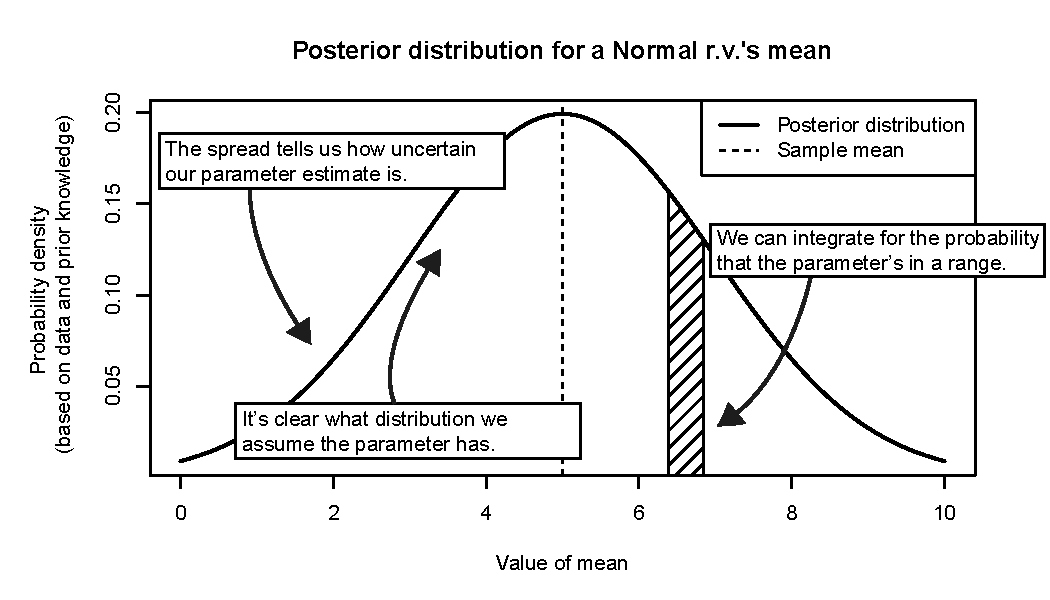
\includegraphics[width=\textwidth]{annotated_posterior.pdf}
\caption{An annotated posterior distribution.}
\label{fig:annotated_posterior}
\end{figure}
\par
Bayesian methods would be useful to DCA because they are easier to understand, visualize, and explain than classical methods\footnote{``Classical methods'' here refers to tools such as hypothesis tests and interval estimates.}, and are relevant to a broader range of situations. They also allow expert knowledge to be used, making it possible to reach a sanitary comprimise between gut-feel and experimental observation. Finally, their emphasis on distribution rather than point estimates better reflects the underlying uncertainty in analytical results. These claims will  be explained in the context of an example.
\par
The proportion of units passing a test is a useful measure of a design's quality. Using the results from a test sample and the expertise of an engineering team, and Bayes' theorem, it is possible to estimate what pass rates would be likely if the design were to be produced in larger volumes.
\par
Say that a sample of $n$ units are tested, and $y$ pass. The engineering team collude to sketch out a distribution for the passing rate $\theta$ that's tall near values they think probable and low near ones that seem unlikely. The team is to calculate the probability of a unit passing, given their experimental data and preliminary distribution: Bayes' theorem can be used to do this.
\begin{equation}
  p(\theta|y) = \frac{p(y|\theta)\cdot p(\theta)}{\int_{\theta}p(y|\theta)\cdot p(\theta)\cdot d\theta}
  \label{eq:bayes}
\end{equation}
In words, this means that a passing proportion is more probable if it makes the the number of units that really did pass in the sample more likely and seems sensible to the engineering team. The denominator of this expression is constant w.r.t. $\theta$, making it possible to express the above as:
\begin{align}
  p(\theta|y) &\propto p(y | \theta)\cdot p(\theta)   \label{eq:unnorm_bay} \\
  \small{\texttt{Posterior}} &\propto\small{{\texttt{Likelihood} \cdot \texttt{Prior}}} \nonumber
\end{align}
(\ref{eq:unnorm_bay}) makes it clear that to estimate $p(\theta|y)$, two things are used:
\begin{itemize}
\item The probability of the data - y in n units passing - given a particular population passing proportion, $p(y|\theta)$ (the \emph{likelihood}).
\item  The probability of a passing proportion according to the engineerig team, $p(\theta)$ (the \emph{prior}).
\end{itemize}
In this case, the likelihood is the probability of $y$ units passing and $(n-y)$ units failing. Assuming that passes and failures and independent and that the units come from the same population, then the probability of $y$ passes given that $\theta$ of that population would pass is:
\begin{gather}
  p(y|\theta) = \binom{n}{y} \theta^y (1 - \theta)^{n - y}
  \label{eq:binom_likelihood}
\end{gather}
In a more general sense, the likelihood is the probability of observing the data given that it was being generated according to the model parameterized by $\theta$.
The prior distribution, $p(\theta)$, encodes knowledge of what passing proportions are probable. If the engineering team is unsure what the passing proportion would be, then they may assume that all values are equally likely:
\begin{equation}
  p(\theta) = 1 \qquad \theta \in [0, 1]
  \label{eq:unif_prior}
\end{equation}
Figure \ref{fig:binom_bayes_inference} displays these prior and likelihood distributions. At this point the engineering team can do one of two things: they can evaluate the posterior analytically, or approximate it using a computer. Irrespective of the method chosen, the expression being evaluated is:
\begin{equation}
	p(\theta|y) = \texttt{constant}\cdot p(y|\theta) \cdot p(\theta)
	\label{eq:example_bayes}
\end{equation}
In practice, (\ref{eq:example_bayes}) is calculated using a computer. A grid of $\theta$ values is defined, and their prior probabilities and likelihoods are calculated in line with the functions in (\ref{eq:unif_prior}) and (\ref{eq:binom_likelihood}). This process can be described by the pseudocode:
\begin{align*}
  \quad n &:= \small{\texttt{No. of units tested}} \\
   \quad y &:= \small{\texttt{No. of units that passed}} \\
  \boldsymbol{\theta} & := (0, \ 0.01, \ \dots, \ 1) \\
  \small{\texttt{Prior}} &:= \small{\texttt{Uniform}}(\boldsymbol{\theta}, [0, 1]) \\
  \small{\texttt{Likelihood}} &:= \small{\texttt{Binomial}}(y, n, \boldsymbol{\theta}) \\ 
  \small{\texttt{Posterior}} &:= \small{\texttt{Prior} \odot \texttt{Likelihood}}
\end{align*}
Where $\texttt{Uniform}$ returns the probability density of the uniform distribution for each value in $\boldsymbol{\theta}$ (i.e. a list of ones), $\texttt{Binomial}$ returns the probability of $y$ in $n$ units passing given each of the passing probabilities in $\boldsymbol{\theta}$, and $\odot$ is the element-wise product.
The posterior list would contain the probability density for each passing proportion $\theta$, and is again shown in Figure \ref{fig:binom_bayes_inference}. The peak indicates more probable values - a taller, pointier peak represents a more certain estimate because a few values have a much higher probability than lots of others. In the same spirit, the flat prior that was used can be understood as highly uncertain.
\begin{figure}
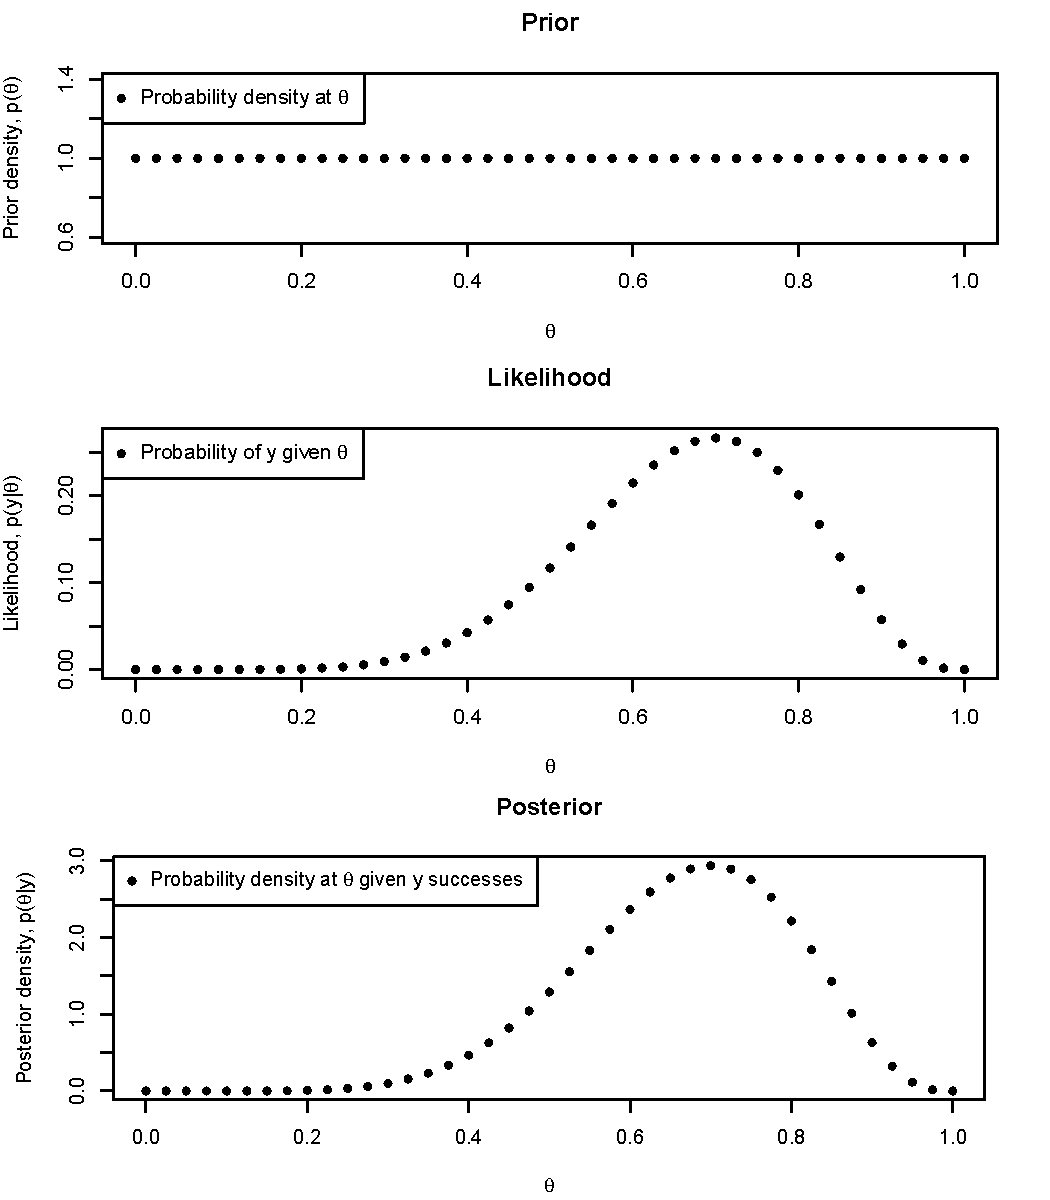
\includegraphics[width=\textwidth]{Bayesian_inference.pdf}
\caption{Combining an uninformative prior with a likelihood distribution to form a posterior distribution of plausible parameter values.}
\label{fig:binom_bayes_inference}
\end{figure}

Once the posterior has been calculated, it can be used to predict the behaviour of future units. $\tilde{y}$ denotes the number of future units that pass, $\tilde{n}$ is the number of units tested. The probability of $\tilde{y}$ successes, based on the observed data and additional information, is the weighted average of $\tilde{y}$ successes over all possible values of $\theta$:
\begin{equation}
	p(\tilde{y}|y) = \int_{\theta}p(\tilde{y}|\theta, y)\cdot p(\theta|y) \cdot d\theta
\end{equation}
Once again, we can avoid some potentially mischievous mathematics by approximating this integral using a computer: draw samples of $\theta$ based on $p(\theta|y)$, then sample a value of $\tilde{y}$ from $p(\tilde{y}|\theta, y)$. Do this many times and the relative frequency of $\tilde{y}$ values will tend towards $p(\tilde{y}|y)$.
\begin{align*}
\small{\texttt{for (i in [1, 10 000]) \{}} &\\
	\tilde{n} &:= \small{\texttt{No. future units to be tested}} \\
	\boldsymbol{\tilde{y}} &:= (0, 1, \dots, \tilde{n}) \\
	\theta &:= \small{\texttt{Sample(}}\boldsymbol{\theta}\small{\texttt{, Posterior)}} \\
	\small{\texttt{Posterior predictive[i]}} &:= \small{\texttt{Sample(}}\boldsymbol{\tilde{y}}\small{\texttt{, Binomial(}}\tilde{y}, \tilde{n}, \theta\small{\texttt{))}}\\
	&\quad\quad \small{\texttt{ \} }}
\end{align*}
Figure \ref{fig:posterior_predictive} shows a plot of the posterior predictive, along with the $5\%$ lower limit on the number of units that will pass. This limit can be interpreted as a bound on the plausible number of units to pass, according to the evidence,
\begin{figure}
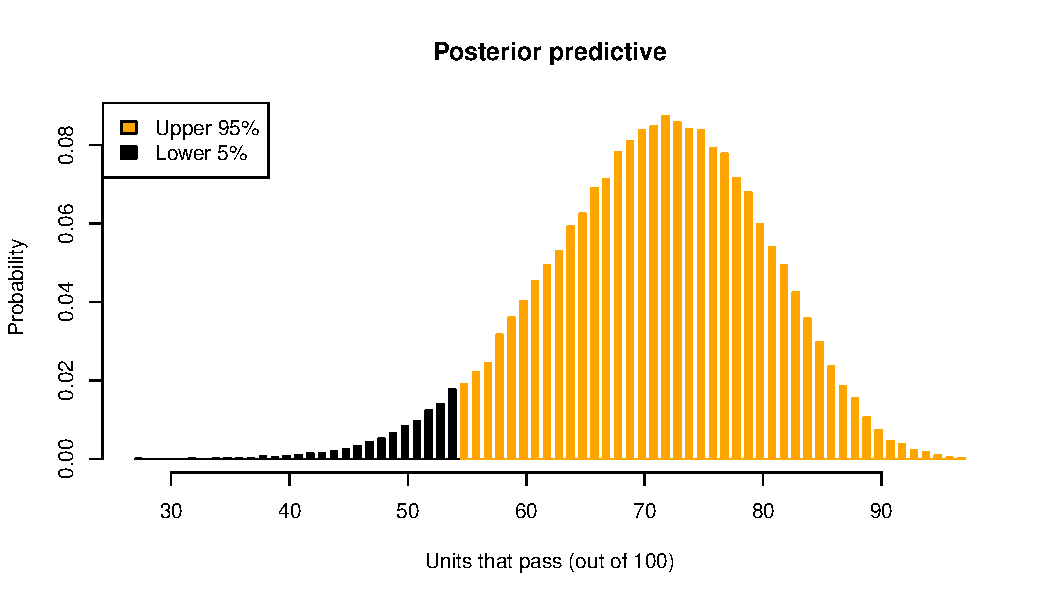
\includegraphics[width=\textwidth]{posterior_predictive.pdf}
\caption{Posterior predictive distribution for the number of passing units in a 100-unit run.}
\label{fig:posterior_predictive}
\end{figure}

The process of inference just described would be valuable to DCA because it would provide a direct representation of how likely particular values are for key performance parameters. Unlike with standard errors, the uncertainty in the estimate is immediately apparent, and the effect of increasing sample size on accuracy is also clear, since the posterior of one analysis can be used as the prior of the next: this means that the information from tests is able to accumulate. This principle is shown in Figure \ref{fig:updating_posterior}, where the flat prior represents initial ignorance about whether a unit will pass: as more units are run, an increasingly narrow peak forms around the most probable passing probability.
\begin{figure}
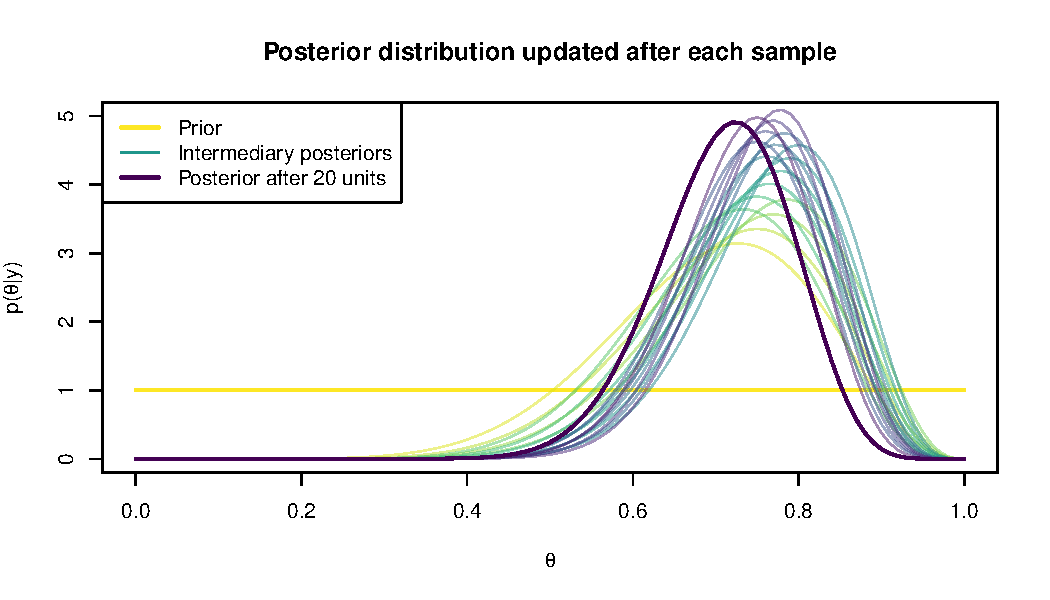
\includegraphics[width=\textwidth]{updating_posterior.pdf}
\caption{The uncertainty in the posterior decreases as more samples are conditioned upon.}
\label{fig:updating_posterior}
\end{figure}
\par

Another advantage of Bayesian methods over hypothesis testing is that it is relatively easy to build models that estimate many parameters simultaneously. An instance of this might be when estimating the mean and the variance of data that's assumed to have a normal distribution. The only change relative to the single-parameter scenario is that we need to define the prior and likelihood in Equation \ref{eq:unnorm_bay} over two parameters instead of one:
\begin{equation}
	p(\theta_1, \theta_2 | y) \propto p(y|\theta_1, \theta_2) \cdot p(\theta_1, \theta_2)
\end{equation}
Where $\theta_1$ is the data's mean, $\theta_2$ is its standard deviation, and $y$ is the dataset. Using a joint prior that weakly favours a range of mean and variance values (based on sensible physical estimates) and a normal likelihood $p(y|\theta_1, \theta_2) = \text{N}(\theta_1, \ \theta_2^{\ 2})$ results in a distribution of parameter values like that shown in Figure \ref{fig:multiparameter_bayes}. This distribution shows how the data reduced uncertainty about what values are reasonable for the mean and standard deviation. This distribution would probably be easier to explain to clients and colleagues than confidence intervals or hypothesis tests.

\begin{figure}
\centering
\makebox[0pt]{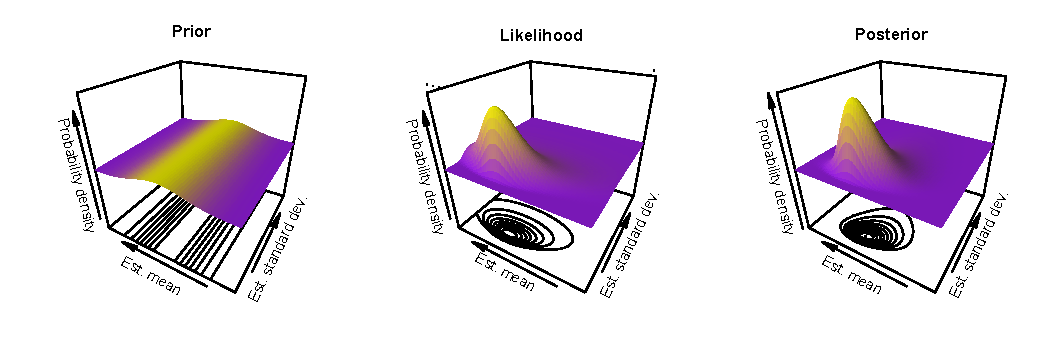
\includegraphics[width=1.4\textwidth]{multiparameter_bayes.pdf}}
\caption{Multiparameter Bayesian inference.}
\label{fig:multiparameter_bayes}
\end{figure}

Shifting from classical methods to Bayesian ones would make statistics within DCA more transparent to both its engineers and clients. Hypothesis tests and interval estimates are easily misinterpreted and are opaque representations of the certainty in parameter estimates, since they are presented simply as numerical values. The jargon of classical statistics can make it unclear what's relevant to the problem, and makes an honest explanation of its methods to non-technical team members difficult. Bayesian methods make it clear how the data and prior knowledge are being combined, and provide results that are easier to interpret. On the other hand, sophisticated Bayesian models require careful thought to be applied effectively, and  may take longer to set up as a result. However, a couple of models could probably answer most questions asked in experimental work, such that once a model is set up it can be used to analyze data from many different experiments.
\par
It is generally recognized that the scientific community as a whole needs to reconsider the practical relevance of hypothesis testing: DCA can hardly be faulted for neglecting to apply ineffective methods. Tolerance and confidence intervals are useful, but can be prone to misinterpretation. 

\section{Experiment Design}
Experiment design is motivated by trying to find efficient ways to explain response variation. Attributing response variation to product factors is the first step towards tuning those factors to produce a desirable response. Response surface methodologies would allow DCA's engineers to do this.

\subsection*{Response Surface Methodologies}
In any given one of DCA's products, it is likely that most parameters will either need to be:
\vspace{-14pt}
\begin{itemize}
	\item Kept within a range - for example, criticial dimensions, or
	\item Maximized/minimized - such as mechanism friction or split line prominence.
\end{itemize}
\vspace{-14pt}
Response surface methodologies (RSMs) try to achieve these objectives by sequentially identifying the factors that affect the response parameter. The factors that have the biggest effect on the response are measured and approximately optimized first. Once this has been done, subtler effects - such as factor interactions - are explored, allowing the system to then be optimized with respect to all factors. Figure \ref{fig:RSM_overview} is included to support this explanation \cite{montgomery2000design}.
\begin{figure}[h!]
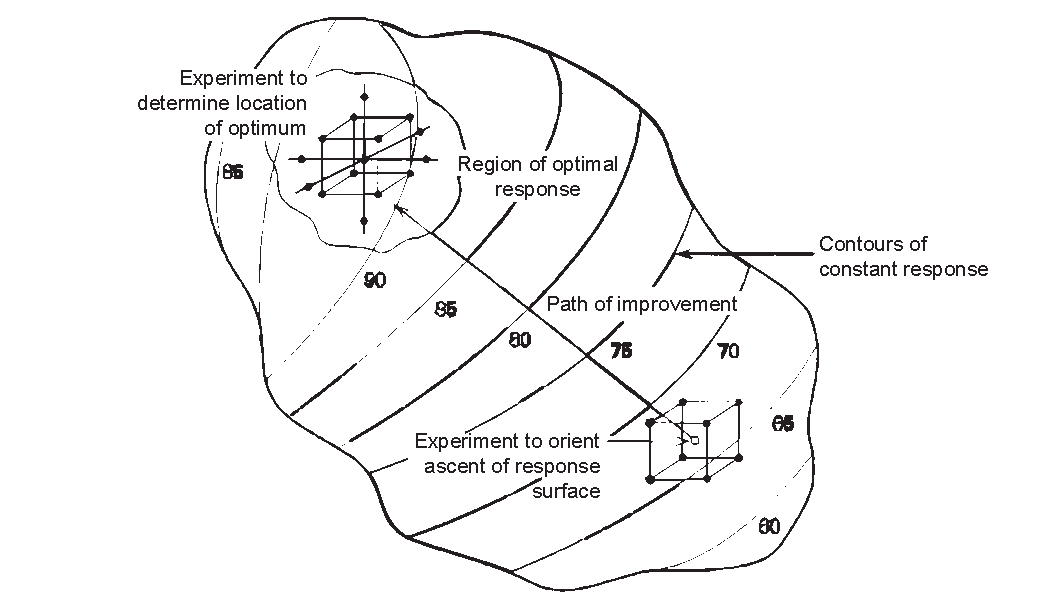
\includegraphics[width=\textwidth]{RSM_overview.pdf}
\caption{RSMs progressively optimize a system's response.}
\label{fig:RSM_overview}
\end{figure}

Response surface methodologies are built around linear models. The link is clearest when an RSM is broken down into steps:
\begin{enumerate}
\item Start by determining what the first-order effects of factors are on the response. In other words, estimate the coefficients $\beta_i$ in the model:
\begin{equation}
	f(x_1, ..., x_n) = \beta_0 + \sum_{i = 1}^n \beta_i \cdot x_i
\end{equation}
\item Incrementally optimize the response based on the model. If the response were being maximized, this would mean adjusting the factors $x_i$ until the reponse $f(x)$ stops increasing. 
\item Determine what the second-order interaction effects are in the vicinity of the first-order optimum. That is, fit a model of the form:
\begin{equation}
	f(x_1, ..., x_n) = \beta_0 + \sum_{j = 1}^n \beta_{j} x_j + \sum_{i = 1}^n \beta_{ii} x_i^2 + + \sum_{i = 2}^n \sum_{j < i}\beta_{ij} x_i x_j
\end{equation}
\item Optimize the response according to these second-order effects.
\end{enumerate}
Something missing from the above steps is that factors that have a negligible effect on the response need to be discarded to avoid having to test a staggering number of second-order treatments to test.

A 2-level factorial design can be used in step (1). This design provides enough information to estimate the intercept, main effects, and interaction effects - the left panel of Figure \ref{fig:rsm_design} explains this in detail. By using center points, it's possible to estimate the response variance and to check whether there is any curvature in the response surface. The test for curvature is quite simple: if the response at the center point is substantially above or below the response plane described by the boundary points, then it suggests that the response surface in the region is curved. Curvature implies that quadratic (or possibly even higher order) effects are important to the response's variation.

At the second step, where the response is optimized in the vicinity of the optimum, more points need to be taken in order to estimate the quadratic effects. To estimate these, three points along each factor's axis are needed. The design shown in the right panel of Figure \ref{fig:rsm_design} does exactly this: the outer elements can be used to estimate curvature (averaged across two paths), while the center point can be used to estimate error in the region of interest.
\begin{figure}
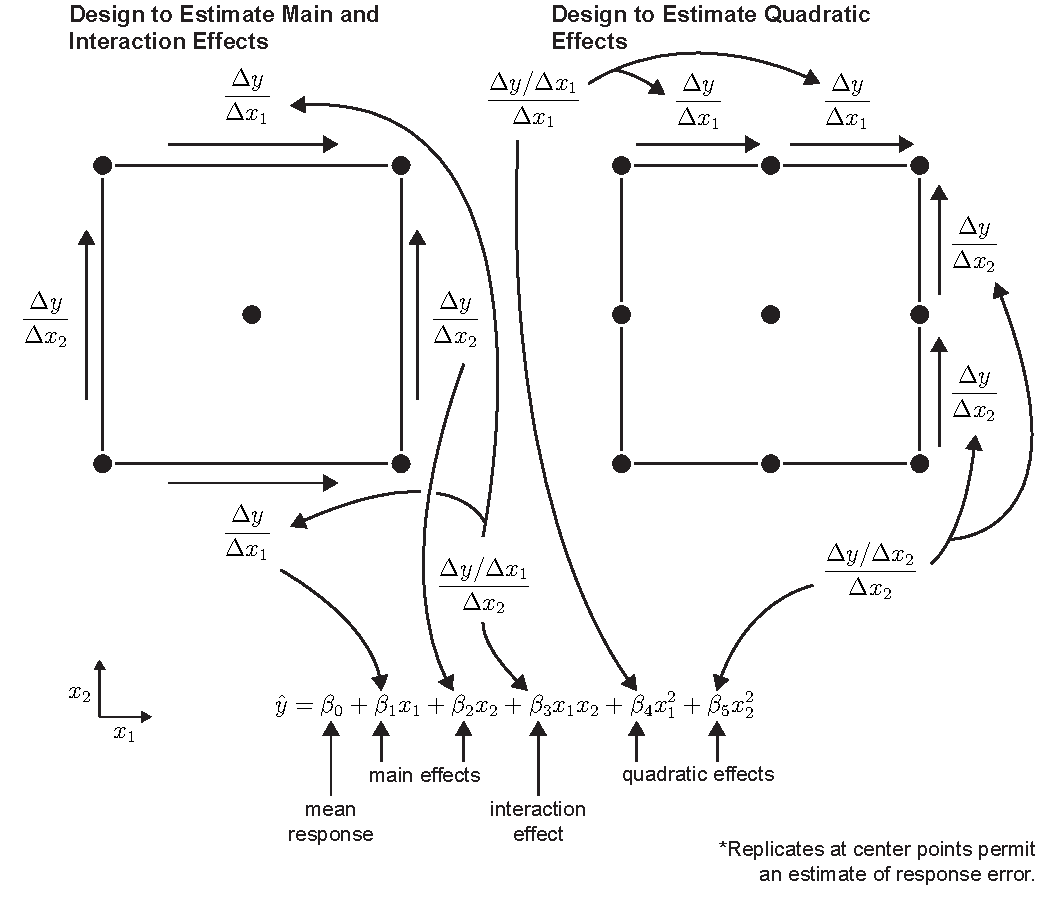
\includegraphics[width=\textwidth]{RSM_design.pdf}
\caption{Left}
\label{fig:rsm_design}
\end{figure}

RSMs would converge on solutions more quickly than DCA's current best-guess approach, and would optimize product performance. It can be difficult obtain the resources to run a large experiment, and to convince a client that it will be worthwhile, but perserverance will repay itself in the risk avoided and quality gained as a result. Investigations relying on expert guessing will tend to consume more resources than planned investigations. This design provides an idea of the minimum cost to understand the effects of a set of factors on a response. If this cost is too high, and the factors can't be reasonably discounted, then the objectives of the investigation should be refined.

\newpage
%%
\section{Visualization}
\label{suggested_vis}
Good visualization exposes patterns in data in a way that's immediately interpretable and precise. A visualization is a mapping from the numerical domain of a dataset to the visual domain of a plot. Data isn't stored in a way that can be interpreted easily, so it needs to be transformed for it to be useful - mathematics is one means of transforming it to reveal patterns, and plots are another.

Designing a visualization means giving thought to:
\begin{itemize}
\item Data - are the variables continuous, categorical, or ordered categorical?
\item Geometry of datapoints - points, lines, or bars.
\item Datapoint aesthetics - color, size, shape, and position of the geometries.
\item Scales - mappings from data to aesthetics.
\item Summary statistics - plottable summaries of the data.
\item Facets - plotting subsets of the data separately.
\item Themes - typeface, non-data colours, axes and so on.
\end{itemize}
This many elements may seem overwhelming, and can be justified, but the most important are choice of geometry, aesthetics, and scales. Aesthetics can represent dimensions that are not displayed via a plot's axes: group membership, for example, is often depicted by a datapoint's colour or shape. Datapoint geometry, meanwhile, carries information such as resolution, chronology, and connectivity. Lines alone may obscure the sampling rate in a time series, and suggest some form of relationship or order between points. Bars are often used to represent an accumulated quantity (such as frequency), whereas points have the capacity to convey information about density and the number of measurements made. Scales describe how to map from numerical values in a dataset to an aesthetic's property. Consequently, scales affect a reader's perception of gradients and ordering. Several scales are shown in Figure \ref{fig:scales}.
\begin{figure}[h!]
\centering
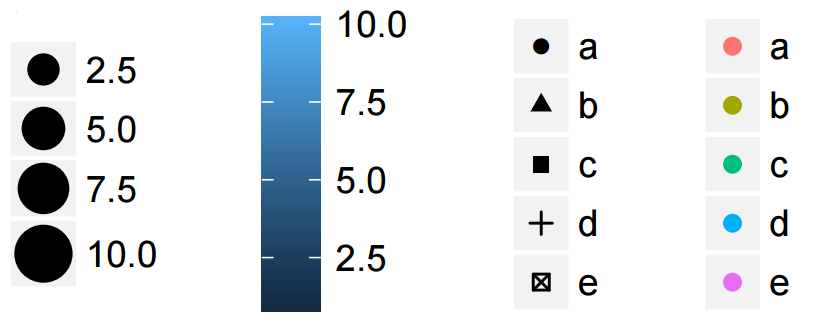
\includegraphics[width=0.6\textwidth]{scales.png}
\caption{Scales describe how to map from numeric values to aesthetic attributes such as shape, size, and colour.}
\label{fig:scales}
\end{figure}
\vspace{-14pt}

To show how the elements listed above provide a framework for presenting data, consider the following example. In DCA, experimental results are regularly discussed in team meetings. These discussions are guided by charts of the results; the conclusions of these meetings will guide an experimental investigation, and can only be as well-informed as those charts permit. If charts contain irrelevant or misleading information, an investigation may stall.
  While default options in programs like Excel and Matlab can be very useful for quickly surveying data, they are rarely ideal for focusing technical discussions. More generally, the same applies to plotting raw time series data directly - gross structure can be made apparent, but there will almost certainly be both a clearer way to express key results.
  
  Figure \ref{fig:imitation_line_chart} is an example of how DCA currently summarizes test data. In this case, the performance of each unit at 10.8 seconds needed to be known. The behaviour of the units over the rest of the time span was thought to provide information as to why there were differences at that point. Each group had a distinct waveform and within groups the waveforms were similar. The shortcomings of presenting raw data directly were discussed in Subsection \ref{sec:dca_vis} - gross structure can be made apparent, but relevant information is otherwise subsumed by noise.
  
   \begin{figure}[h!]
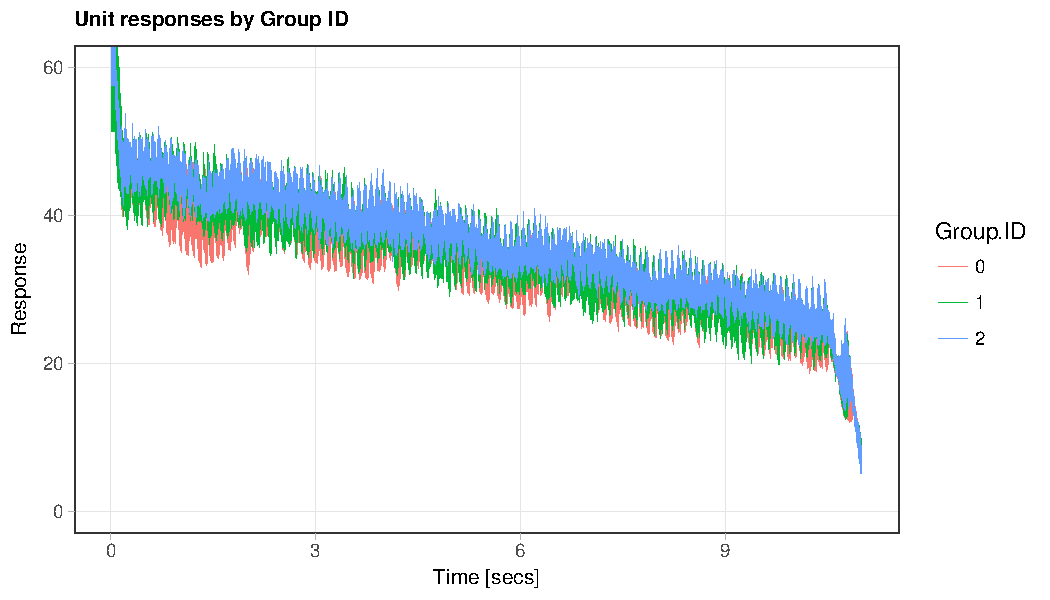
\includegraphics[width=\textwidth]{imitation_line_chart.pdf}
\caption{}
\label{fig:imitation_line_chart}
\end{figure}
  
   Figure \ref{fig:better_chart} shows how splitting out specific observations into separate charts would have allowed this experimental data to be understood more deeply\footnote{The response units have been witheld to preserve confidentiality.}. Each of its charts is facilitates a specific technical discussion, but also provides information that supports the questions posited by its neighbors. The second chart, a strip plot, focuses on a key measure of each group's performance. The number of units tested is shown by this plot, as is the spread in the response, two pieces of information that are valuable to a reader because they measure a test's precision. Including the group sample means also prevents outliers skewing how the groups relative performance is perceived. The colours mapped to each group in these first two plots are of a similar intensity and are colorblind-safe. Using colors of a different luminance\footnote{Luminance is a measure of a surface's brightness.} can unintentionally skew attention towards a particular datapoint or group. Additionally, the colors chosen did not have a perceptual ordering, as say a sequence of red shades would: this is important since there was no natural ordering to the group treatments in the experiment.
   
 The final plot uses color to emphasize an observation, and provides a diagram so that the physical system under study can be related to the experimental data. As with the first plot, an annotation states the message being conveyed.
\begin{figure}
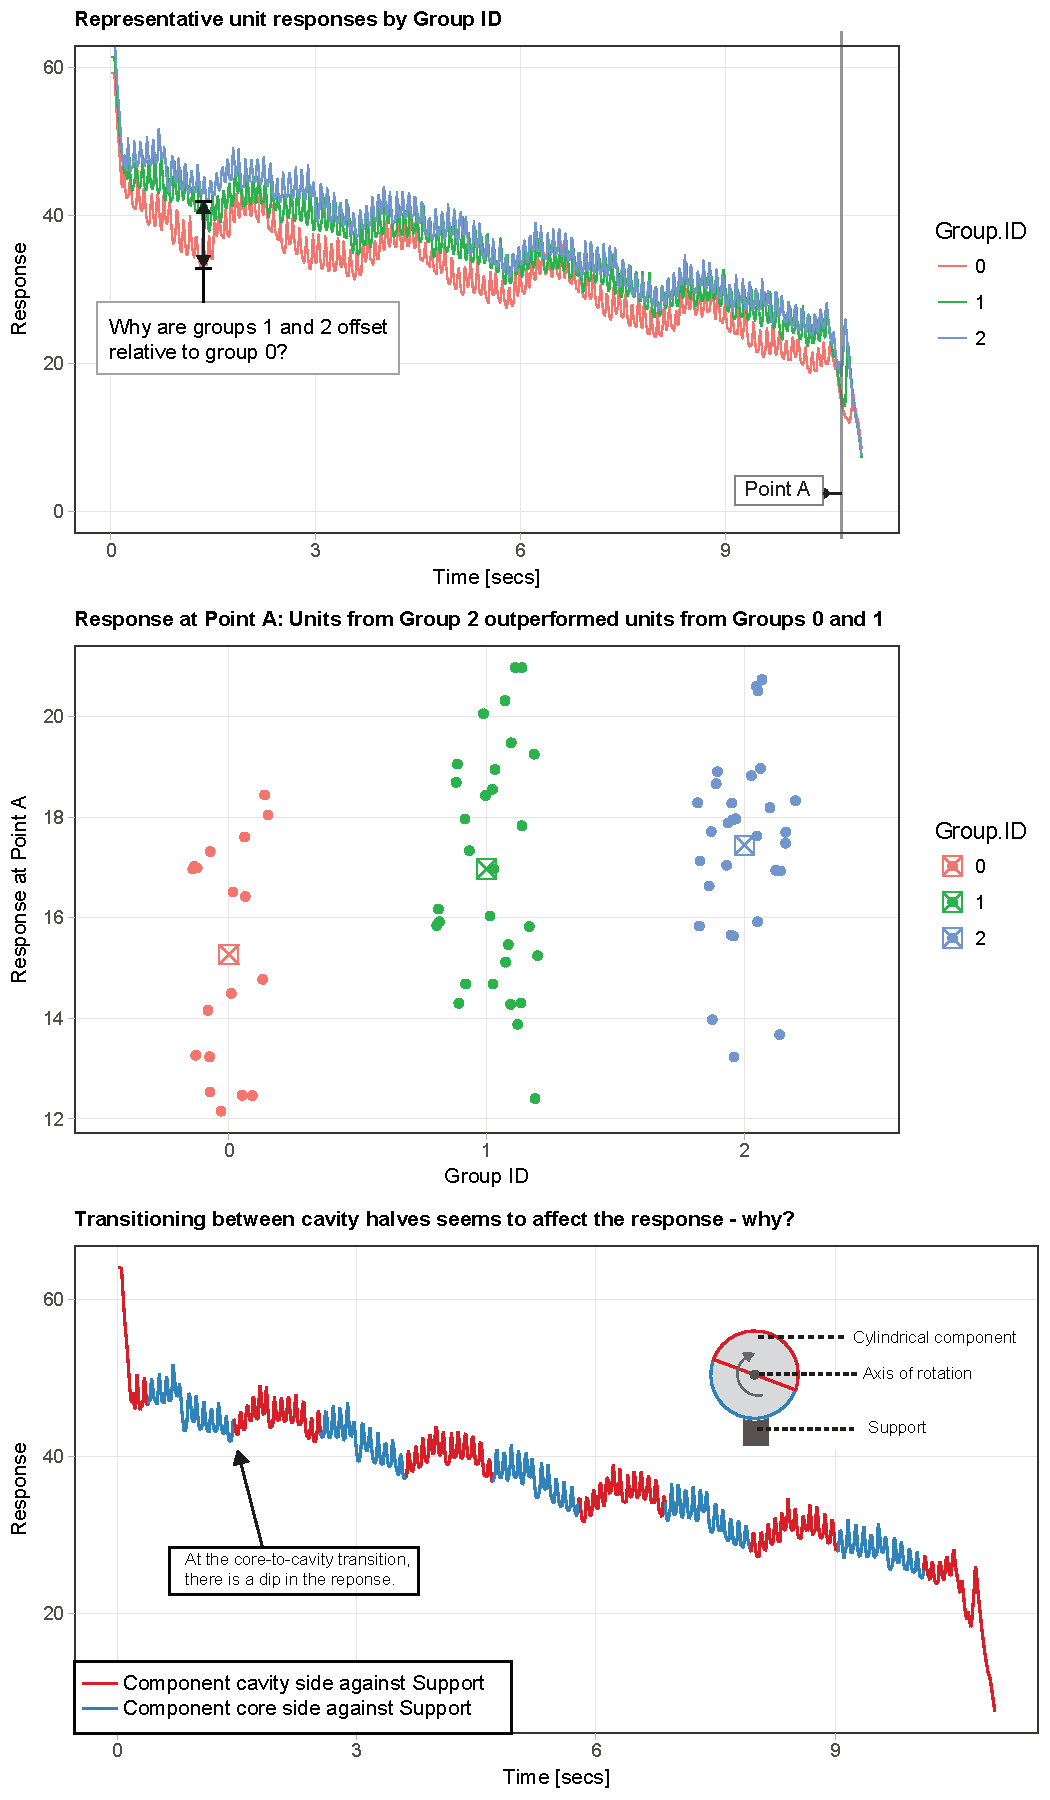
\includegraphics[width=\textwidth]{better_charts.pdf}
\caption{}
\label{fig:better_chart}
\end{figure}

This example stresses that if graphs are used to direct technical discussions then they should form a narrative. If a particular result is of interest then that result should be abstracted into as simple a plot as possible. Properties affecting the precision of an experiment - such as its size and controls - can be embedded in a plot through aesthetics, geometry, facets, and scales. Where needed, diagrams and annotations should be used to provide the information needed to understand the plot. Applying these principles would make it easier for DCA's engineers to discern nuanced patterns and present their findings to their colleagues and clients.

A relevant topic here is jet colormap, the default used by many of DCA's simulation packages. This colormap has been criticized as being actively misleading and confusing. Luminance allows the visual system to perceive boundaries; across the jet colormap, luminance does not change at a constant rate. In some sections it changes very rapidly, whereas in others it is almost constant. This has the dual effect of suggesting sharp boundaries where they may not exist in the data, and obscuring actual borders in the map's isoluminant regions. Figure \ref{fig:jet} demonstrates these qualities.
\begin{figure}
\centering
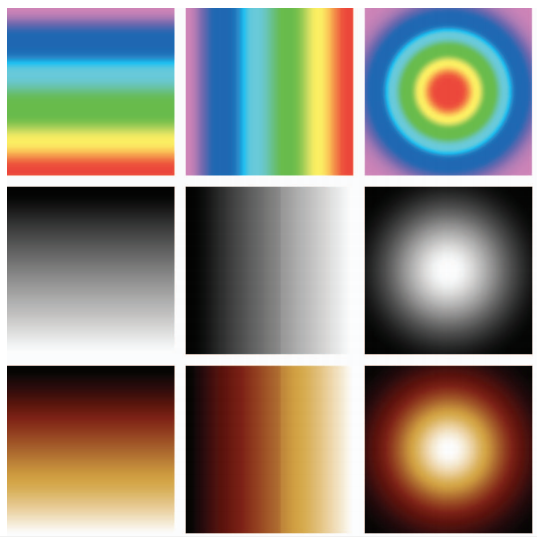
\includegraphics[width=0.5\textwidth]{jet.png}
\caption{\small{Each column corresponds to a set of data. Column 1 is a vertical linear scale; 2 is linear with a step at the center; 3 maps radius. Grayscale and black-body colormaps accurately represent the underlying data: jet does not.}}
\label{fig:jet}
\end{figure}

\cite{hastie2013elements}, \cite{gelman2013bayesian}, \cite{faraway2004linear}, \cite{blitzstein2014linear}, \cite{jaynes2003probability}, \cite{wickham2009ggplot2}, \cite{montgomery2000design}, \cite{kruschke2015doing}, \cite{iso2014statistical}, \cite{borland2007rainbow}.


%%
\section{Software}
 Software is required to implement the tools presented. Excel and Matlab are already at use within DCA. The company also owns a Minitab license. Ideally, the software would be:
 \begin{itemize}
 \item Easily learnt - can be picked up without requiring specialist training.
 \item Powerful - provides tools for implementing the methods presented.
 \item Succinct - generates results quickly.
 \item Readily understood by other engineers and clients, possibly via reporting tools.
 \item Inexpensive.
 \end{itemize}
\par
 Excel is an excellent tool for quickly plotting test results, but it can only be used for basic analyses and plotting. Its tools for filtering data are clumsy in comparison to those provided by Matlab and R. Moreover, it is prone to slowdown when large datasets are being handled. That said, it requires no previous programming experience to use, which is a signficant advantage when results need to be passed on to clients. Excel does not provide tools for experiment design, linear modelling, or Bayesian analysis.
\par
Matlab's tools for statistical analyses are contained within Mathworks' Statistics and Machine Learning Toolbox. For the analytical methods presented here to be used, this Toolbox would be necessary. To use it, the company would need to invest at upward of £1800 per year\footnote{ An individual annual Matlab license costs £1800, with the Toolbox costing an additional £900. DCA already own five networked licenses (these are more expensive than individual licenses).}. DCA's graduate engineers are already familiar with Matlab, and do much of their mathematical modelling in the software. Consequently, Matlab may make it easy to integrate statistics into DCA's existing simulation work. Furthermore, Mathworks offer tools tailored to specific engineering tasks. Matlab's documentation also tends to be clearer, and its debugging tools are very good.
\par
R is an open-source programming language designed for statistics. It is free to use, as are its many extensions which provide advanced modelling, visualization, and data-manipulation tools. Academic researchers and professional analysts rely on R for their work, reflecting the fact that R is held to be the standard tool for statistical analysis. All of the plots in this report were produced using R, some of which would have been difficult to produce using Matlab; R offers data-reshaping tools that Matlab does not, and has an exceptionally flexible plotting extension. RStudio, a free development environment, also provides tools for automatically formatting analyses into PDFs or webpages. A major drawback to using R is that it has quite a steep learning curve. This is in due to its unusual syntax which can make code difficult to read, and the cryptic error messages that result from its ability to store different data types in one variable. As an estimate, it would probably take one of DCA's engineers at least 20 hours to become familiar enough with base R to use it to run the analyses presented here. This would cost at least £1200, but would be a one-time investment (per engineer). 
\par
Minitab costs £1300 per license and provides a graphical interface for designing and analysing experiments. It guides the user towards appropriate experiment designs and analyses based on their needs, but is less flexible and extensible in comparison to Matlab and R's. Its tools for filtering and reformatting data are also, by comparison, limited. It may be the most approachable choice here, besides Excel, for engineers without prior programming experience.
\par
As is probably clear, no one software package stands out as being exceptionally well-suited to the company's needs.

%% CONCLUSIONS AND RECOMMENDATIONS %%
\chapter{Conclusions \& Recommendations}
\vspace{-28pt}
Statistics allows engineers to:
\begin{itemize}
\item Design robust products.
\item Optimize product performance.
\item Minimize risk in product development.
\item Conduct efficient experimental investigations.
\item Develop a coherent understanding of a product's behaviour.
\item Present the uncertainty inherent in experimental work honestly.
\end{itemize}
It is for these reasons that DCA should continue to develop its expertise in statistics. Professional experimental work is necessary to deliver high-quality products. Statistical expertise is pre-eminently marketable, particularly given the recent surge in popularity of machine learning algorithms. Being able to meet the technical demands of clients int this area would allow DCA to surpass the offerings of other technical product design consultancies: statistics provides a lucid approach to product development that is uniquely able to handle risk and meet strict performance criteria. Asking DCA's engineers to become statisticians is unrealistic: engineers are paid to deliver products, not to study. Consequently, it may be advisable for the company to hire a statistician or a testing development engineer. DCA's engineers are almost always involved with project work, giving them very little time to prepare the kinds of tools described in this report. A contractor dedicated to enhancing DCA's statistical offering could resolve the company's existing experimental problems, and support the development work of DCA's core engineering staff.

A reasonable criticism of the methods proposed is that products do not need to be optimal, and that experimental investigations do not need to be absolutely efficient. This is true - they do not. Products can be ``good enough''. However, neglecting to develop a coherent view of a product's performance in the face of manufacturing and environmental variation exposes projects - and therefore the company - to severe risk. DCA claims to strive to ``deliver market-leading products through world-class engineering''. As clients demand increasingly sophisticated products, DCA's engineers will need tools to manage mounting complexity and uncertainty, particularly if they wish to match up to this bold claim. Statistics can provide some tools that they would find useful.


\newpage
%% BIBLIOGRAPHY
\bibliographystyle{plain}
\bibliography{icr}

\newpage
%% APPENDIX %%
\appendix
\chapter{}
\subsection{What is probability theory, and what is a probability?}
Probability allows us to analyze a system without requiring complete mechanical knowledge of it. `'Randomness'' refers to sources of variation that are not measured. You may have heard of probabilities as representing `'Degrees of belief''. To understand what a belief is, consider this example. We machine a coin that we check is a symmetric disk of homogeneous density. I flip the coin ten times, and it comes up heads every single time. You might be surprised by this, and accuse me of flipping it in a controlled way. I then ask you how I can flip it in a way that is fair. What is your response?
\par
If you say that it should come heads as many times as tails, then the experiment is no longer random, as we know what the outcome will be. You may gesticulate and say ``You need to flip it \emph{randomly}''. I would press you to tell me what this means - I require a mechanism to decide how to flip the coin, and physical mechanisms are deterministic.
\par
Point being, the probability of an outcome can only be evaluated relative to a set of assumptions you make about the mechanism generating those outcomes. You had a preconceived notion that the way I flipped the coin would favor neither heads nor tails, and therefore saw ten heads as supremely improbable. It is exactly these kinds of assumptions that form the basis of statistical analyses. Being able to express physical assumptions mathematically gives an analytical voice to our physical understanding of the world, and should ideally feel as natural as that understanding.
\newpage

\subsection{Standard Error of a Sample Mean}
We can see this by recognizing that the sum of independent observation's variances is equal to the variance of the sum of the observations:
\begin{align}
 \text{Var}\sum_{i = 1}^n X_i &= \sum_{i = 1}^n \text{Var}X_i\\
	\text{Var}n\bar{X} &= n\text{Var}X \\
	\implies \sqrt{\text{Var}\bar{X}} &= \frac{\sigma}{\sqrt{n}}
\end{align}
\par
Analytically, we can solve for $p(\theta|y)$ directly
\[
  p(\theta|y) \propto \binom{n}{y}\theta^y (1 - \theta)^{n-y}\cdot 1
\]
To find the constant of proportionality, we need to divide the r.h.s. by its integral over all values of $\theta$, such that the $\int_0^1 p(\theta|y)\cdot d\theta = 1$. As it happens, the r.h.s. has the form of what's called a beta distribution
\[
  p(x; a, b) \propto x^{a - 1}\cdot x^{b-1}
\]

\subsection{Confidence intervals}
\begin{align}
	\text{P}(\bar{x} - ks \leq \mu \leq \bar{x} + ks) &= 1 - 2\cdot \text{P}(\bar{x} - ks \leq \mu) = 1 - \alpha \nonumber\\
	\implies \frac{\alpha}{2} &= \text{P}(\frac{\bar{x} - \mu}{s} \leq k) 
\end{align}
The last line implies that $k$ has a $t$-distribution with $n - 1$ degrees of freedom, so that the confidence limit that contains the true mean $(1 - \alpha)\%$ of the time is
\begin{equation}
	[\bar{x} - t_{n-1}(\alpha)\cdot s, \ \bar{x} + t_{n-1}(\alpha)\cdot s]
\end{equation}
\[
	 = \text{P}\Bigg(\frac{\Big(\frac{\bar{x} - \mu}{\sigma/\sqrt{n}}\Big)}{s/\sqrt{n}\sigma}\Bigg)
\]


\subsection{Justifications for Least-Squares Regression}
\begin{gather}
	\text{Assume that the errors in $y$ given $x$ are normal with constant variance and mean zero}\\
	\epsilon \sim \text{N}(0, \sigma^2) \\
	p(\epsilon|\hat{\beta}) = \frac{1}{\sqrt{2\pi}\sigma} \exp (-\frac{\epsilon^2}{2\sigma^2})
\end{gather}
Assume that the true response is a linear function in $\hat{\beta}$, such that $E(Y|X) = X\hat{\beta}$, then take the log of the likelihood:
\begin{gather}
	l(\hat{\beta}) \propto -(Y - X\hat{\beta})^2
\end{gather}
Such that maximizing the likelihood is equivalent to minimizing the RSS criterion.

The final way to justify a least squares fit does not require a normality assumption: instead, it is rationalized as providing the lowest variance estimate of $EY$ for a given $X$. In other words, a least squares fit will, on average, be closer to the true response than a linear fit made in some other way.

Start by assuming that $y$ truly is a linear function of $X$, which is a vector of inputs, so that:
\begin{gather}
	E[y|X] = X\hat{\beta} 
\end{gather}
Next note that it follows from the above that the least squares fit will be an unbiased estimate, provided that $\boldsymbol{y}$ is drawn i.i.d. at a given $X$:
\begin{gather}
	E[X\hat{\hat{\beta}}] = E[\boldsymbol{X(X^T X)^{-1}X^T y}] \\
	= \boldsymbol{X(X^T X)^{-1}X^T X}\hat{\beta} \\
	\implies E[X\hat{\hat{\beta}}] = \boldsymbol{X}\hat{\beta}
\end{gather}
Almost there. Now we need to think about other possible estimates of $E[y|X]$. We can see from (16) that our estimate is a linear function of $y$ (Estimable functions?). Imagine another function $\boldsymbol{c^T y}$ that's also linear in $\boldsymbol{y}$. The Gauss-Markov theorem states that the variance of the least-squared estimate is guaranteed to be less than this other linear estimate:
\begin{equation}
	\text{Var}(\boldsymbol{X}\hat{\hat{\beta}}) \leq \text{Var}(\boldsymbol{c^Ty})
\end{equation} 
The proof for this is:
\begin{gather}
	E[(a^T \hat{\hat{\beta}} - a^T \hat{\beta})^2] \leq E[((c^T y - a^T \hat{\hat{\beta}}) - ( a^T \hat{\beta} - a^T \hat{\hat{\beta}}))^2]\\
	\leq  E[((c^T y - a^T \hat{\hat{\beta}}) + ( a^T \hat{\hat{\beta}} - a^T \hat{\beta}))^2] \\
	\leq E[(c^T y - a^T \hat{\hat{\beta}})^2] + E[( a^T \hat{\beta} - a^T \hat{\hat{\beta}})^2] \\
	\iff 0 \leq E[(c^T y - a^T \hat{\hat{\beta}})^2]
\end{gather}
Is this is a proof? How can you be sure?

\subsection{Derivation of tolerance intervals}
So tolerance intervals allow us to make statements about the performance of a population, with clear limits on that statement's uncertainty. Tolerance intervals are derived by thinking about the probability that a member of the population will be within a particular range. For a one-sided tolerance limit - a value for which at least $p\%$ of the population is greater than or less than - this means:
\begin{enumerate}
	\item Defining $k$ such that the probability a member of the population $(\mu + u \sigma)$ is greater than $k$ sample standard deviations from the sample mean is equal to $1 - a$.
		\begin{equation}
			P(\bar{x} + ks \geq \mu + u_p \sigma) = 1 - \alpha
			\label{eq:tol_interval}
		\end{equation}
	Where $\bar{x}$ is the sample mean, $s$ is the sample standard deviation, $\mu$ is the true mean of the population, $\sigma$ is its true standard deviation, and $u_p$ is such that $\mu + u_p\sigma$ is greater than $p\%$ of the population. $\alpha$ is the confidence level. \newline In words, $k$ is such that $\bar{x} + ks$ will  be greater than the $p\%$ of the population $(1 - \alpha)\%$ of the time.
	\item Assuming $x$ has a normal distribution then $u_p$ can be read off a table of normal values, and by definition $\frac{(n-1)s^2}{\sigma^2}$ will have a chi-square distribution (see Appendix A). What this means is that $k$ has the same distribution as a $t$-distributed r.v. centered at $\sqrt{n}u_p$ and scaled by $\frac{1}{\sqrt{n}}$:
		\begin{equation}
			k = \frac{1}{\sqrt{n}}t_{n - 1}(\sqrt{n}u_p) 
		\end{equation}
		This is a normal distribution that's more spread out - the bigger spread represents the uncertainty on account of the fact that the true variance isn't known.
	\item  Bonanza! The lower interval containing at least $95\%$  of the population is
\begin{equation}
	\Big(-\infty, \bar{x} + \frac{t_{1 - \alpha}(\sqrt{n}u_p, n - 1)\cdot s}{\sqrt{n}}\Big]
\end{equation}
\end{enumerate}
\end{document}